\documentclass[11pt]{article}
\usepackage{amsmath, amssymb, amsthm, enumerate}
\usepackage[margin=1in, top=1.2in, bottom=1.2in]{geometry}
\usepackage{parskip}
\usepackage[colorlinks=true, linkcolor=blue, citecolor=blue, urlcolor=blue]{hyperref}
\usepackage{cleveref}
\theoremstyle{definition}
\newtheorem{definition}{Definition}[section]
\newtheorem{theorem}{Theorem}[section]
\newtheorem{lemma}{Lemma}[section]
\newtheorem{proposition}{Proposition}[section]
\newtheorem{corollary}{Corollary}[section]
\theoremstyle{remark}
\newtheorem{remark}{Remark}[section]
\newtheorem{example}{Example}[section]
\setlength{\parindent}{0pt}
\setlength{\parskip}{6pt}
\begin{document}

\begin{center}
{\Large\textbf{Mathematical Methods for Classical Mechanics}}\\
\vspace{0.3cm}
{\normalsize\today}
\end{center}
\vspace{0.5cm}


% --- Page 1 ---
% blank page

% --- Page 2 ---
% blank page

% --- Page 3 ---
The content in the image does not contain mathematical definitions, theorems, proofs, or formal statements. Instead, it appears to be course logistics and administrative details. 
---

\begin{itemize}
    \item \textbf{Course Logistics}

    \begin{enumerate}
        \item V.I. Arnold \textit{Mathematical Methods for Classical Mechanics} (2\textsuperscript{nd} Edition) -- Problems.
        \item \textit{Geometry Mechanics} -- Abraham and Marsden
        \item \textit{Classical Mechanics} from Goldstein.
    \end{enumerate}

    \textbf{Grading Scheme}
    \begin{enumerate}[(1)]
        \item Active Participation (Classroom discussion, Google classroom, Campuswire) : 10\%
        \item Quiz 1 and 2 : 20\%
        \item Midsem : 30\%
        \item Endsem : 40\%
    \end{enumerate}

    \textbf{Short talk} : 30 min (Volunteer)

    \textbf{Office Hours}

    \begin{itemize}
        \item Application / Definition / Examples
        \item Slightly easier
        \item Tricky question
    \end{itemize}

    \textbf{Exam Pattern}
\end{itemize}

% --- Page 4 ---
Consider a particle moving along $S^1$.

\[ S^1 = \{(x,y) \mid x^2 + y^2 = 1 \} \text{ is unit circle.} \]

Imagine $S^n = \{(x_1, \dots, x_{n+1}) \in \mathbb{R}^{n+1} \mid \sum_{i=1}^{n+1} x_i^2 = 1 \}$.

\begin{definition}\label{def:no_single_coordinate}
Tcompactness_of_S1}
$S^1$ is compact.
\end{claim}

Consider $f \colon \mathbb{R}^2 \to \mathbb{R}$ defined by
\[ f(x,y) = x^2 + y^2. \]

Observe $f$ is continuous, and $f^{-1}\{1\} = S^1$ and hence $S^1$ will be closed and bounded. By Heine-Borel (in $\mathbb{R}^2$, we will see why this theorem holds for $\mathbb{R}^n$), hence $S^1$ is compact.

\begin{proof}
$\square$
\end{proof}

% --- Page 5 ---
\begin{definition}\label{def:parametrization_s1}
A \emph{parameterization} of the unit circle $S^1$ is given by the map
\[
\gamma \colon \mathbb{R} \to S^1, \quad \theta \mapsto (\cos \theta, \sin \theta),
\]
defined using Taylor series.
\end{definition}

\begin{remark}\label{rem:invertible_smooth_map}
Is there a map $\gamma \colon I \to S^1$ such that $\gamma$ is invertible and differentiable ($C^\infty$), i.e., smooth?
\end{remark}

\begin{proof}
Observe the map
\[
\gamma(\theta) = (\cos \theta, \sin \theta), \quad \theta \in [0, 2\pi].
\]
This does not work as $[0, 2\pi]$ is compact, but $S^1$ is also compact (by the Heine-Borel theorem on $\mathbb{R}^2$).

We cannot use any interval as
\begin{enumerate}
    \item An open interval does not hold, in order to preserve continuity of the map.
    \item A closed interval, the derivative is defined one-sided for end points (not differentiable).
\end{enumerate}
\end{proof}

% --- Page 6 ---
---

Consider the construction of a coordinate system on $S^1$.

Let $P_N$ denote a stereographic projection from $N = (0, 1)$.

\[
P_N \colon S^1 \setminus \{N\} \to \mathbb{R}
\]
\[
(x, y) \mapsto \frac{x}{1 - y}
\]

Write how we get this:

By the two-point formula,
\[
\frac{y - 1}{x - 0} = \frac{1 - 0}{0 - x_0}
\]
where $x_0$ is the $x$-intercept, i.e.
\[
x_0 = \frac{x}{1 - y}
\]

\begin{proof}
Check $P_N$ is bijective.

\[
\ker P_N = \frac{x}{1 - y} = 0 \implies x = 0
\]
\end{proof}

---

% --- Page 7 ---
The kernel of \( P_N \) is given by
\[
\ker P_N = \mathbb{Z}(0, -1)^\top.
\]

We observe that \( P_N \) is injective if and only if \( \ker P_N = \{0\} \), but here we are not obtaining the zero vector. Is \((0, -1)\) similar to "0"?

\begin{proof}
To show that \( P_N \) is surjective, we need to show that \( P_N(S_1 \setminus N) = \mathbb{R} \).

For \( k \in \mathbb{R} \), we want to show that there exists \((x_k, y_k) \in S_1 \setminus N\) such that
\[
P_N(x_k, y_k) = k.
\]
This means
\[
\frac{x_k}{1 - y_k} = k \implies x_k = k(1 - y_k).
\]

Now, since \( x_k^2 + y_k^2 = 1 \), substituting \( x_k \) gives
\[
k^2(1 - y_k)^2 + y_k^2 = 1.
\]
Expanding this, we have
\[
k^2(1 - 2y_k + y_k^2) + y_k^2 = 1,
\]
which simplifies to
\[
(k^2 + 1)y_k^2 - 2k^2y_k + (k^2 - 1) = 0.
\]

The discriminant of this quadratic equation in \( y_k \) is
\[
\Delta_y = (4k^2)^2 - 4(k^2 + 1)(k^2 - 1) = 16k^2 - 4(k^4 - 1) = 16k^2 - 4k^4 + 4 \geq 0.
\]
This implies that \((x_k, y_k)\) exists for all \( k \in \mathbb{R} \).

Therefore, the inverse image of \( k \) under \( P_N \) is given by
\[
P_N^{-1}(k) = \left( \frac{2k}{1 + k^2}, \frac{k^2 - 1}{1 + k^2} \right).
\]
\end{proof}

% --- Page 8 ---
Check construction, and derive the following:

\begin{exercise}
Verify the stereographic projection from $(0, -1)$ and is given by
\[
\begin{aligned}
P_S \colon S' \setminus S &\to \mathbb{R} \\
(\alpha, y) &\mapsto \frac{\alpha}{1 + y}
\end{aligned}
\]
and its inverse
\[
\begin{aligned}
P_S^{-1} \colon \mathbb{R} &\to S' \setminus S \\
t &\mapsto \left( \frac{2t}{1 + t^2}, \frac{1 - t^2}{1 + t^2} \right).
\end{aligned}
\]

Same as $P_N$ given above.

\begin{proof}
\textbf{Construction of $P_N^{-1}$}

Join a line between $(t, 0)$ and $(0, 1)$:
\[
\frac{x}{t} + \frac{y}{1} = 1 \implies y = 1 - \frac{x}{t}.
\]

Substitute in $x^2 + y^2 = 1$, then we get
\[
x^2 + \left(1 - \frac{x}{t}\right)^2 = 1.
\]
Expanding and simplifying,
\[
x^2 + 1 - \frac{2x}{t} + \frac{x^2}{t^2} = 1 \implies x^2 + \frac{x^2}{t^2} - \frac{2x}{t} = 0.
\]
\[
x \left(x + \frac{x}{t^2} - \frac{2}{t}\right) = 0 \implies x = 0 \quad \text{or} \quad x = \frac{2t}{1 + t^2}.
\]
Since $x = 0$ corresponds to the point $(0, 1)$, we take
\[
x = \frac{2t}{1 + t^2}, \quad y = \frac{1 - t^2}{1 + t^2}.
\]
This is similar for $P_S$.
\end{proof}
\end{exercise}

% --- Page 9 ---
Observe that $P_S$, $P_N$ are rational functions and hence differentiable.

\begin{definition}
A map $st \colon P_N$ (or $P_S$) is called a \underline{chart/coordinate system}.
\end{definition}

\begin{definition}
$P_S$ and $P_N$ considered together is called an \underline{atlas}.
\end{definition}

\begin{remark}
$S^1$ admits an atlas consisting of two stationary points $P_S$, $P_N$.
\end{remark}

\begin{proposition}
The composition $P_S \circ P_N^{-1} \colon \mathbb{R} \setminus \{0\} \to \mathbb{R} \setminus \{0\}$ is differentiable.
\end{proposition}

\begin{exercise}
Verify the fact given above. Composition of differentiable functions is differentiable.
\end{exercise}

% --- Page 10 ---
Observe that $P_S \circ P_N^{-1}$ takes $X$ to $Y$, then $(P_S \circ P_N^{-1})^{-1} = P_N \circ P_S^{-1}$ is the inverse of the "change of coordinates."

\begin{enumerate}
    \item \textbf{Exercise:} Generalize the above example to $S^2$ and find the expression for $P_N$, $P_S$, $P_N \circ P_S^{-1}$, $P_S \circ P_N$.

    \begin{definition}\label{def:projection_s2}
        Consider the projections:
        \[
        P_N : S^2 \setminus \{(0, 0, 1)\} \to \mathbb{R}^2
        \]
        defined by
        \[
        (x, y, z) \mapsto \left( \frac{x}{1 - z}, \frac{y}{1 - z} \right).
        \]
        We get the formula from similarity of triangles.
    \end{definition}

    \begin{definition}\label{def:inverse_projection_s2}
        The inverse projection is given by
        \[
        P_N^{-1} : \mathbb{R}^2 \to S^2 \setminus \{(0, 0, 1)\},
        \]
        defined by
        \[
        (x, y) \mapsto \left( \frac{2x}{x^2 + y^2 + 1}, \frac{2y}{x^2 + y^2 + 1}, \frac{x^2 + y^2 - 1}{x^2 + y^2 + 1} \right).
        \]
    \end{definition}

    \item Work out the expression for the case of $S^n$.

    \begin{definition}\label{def:projection_sn}
        Consider the projection
        \[
        P_N : S^n \setminus \{(0, \dots, 0, 1)\} \to \mathbb{R}^n,
        \]
        defined by
        \[
        (x_1, \dots, x_n, x_{n+1}) \mapsto \left( \frac{x_1}{1 - x_{n+1}}, \dots, \frac{x_n}{1 - x_{n+1}} \right).
        \]
    \end{definition}
\end{enumerate}

% --- Page 11 ---
\begin{definition}\label{def:chart}
Given a space $X$, $n \in \mathbb{N}$.
A chart for $X$ is a pair $(U, \varphi)$ where $U$ is an open subset of $X$ and $\varphi \colon U \to A$ is a homeomorphism, where $A$ is an open subset of $\mathbb{R}^n$.
\end{definition}

\begin{definition}\label{def:compatible_chart}
For two charts $(U, \varphi)$ and $(V, \psi)$ are compatible if $\varphi \circ \psi^{-1}$ and $\psi \circ \varphi^{-1}$ are differentiable (and invertible), and $U \cap V \neq \emptyset$.
\end{definition}

\begin{definition}\label{def:atlas}
An atlas is a collection of compatible charts $\{(U_i, \varphi_i)\}_{i \in I}$ such that the union of $U_i$'s contains every point of $X$.
\end{definition}

\begin{remark}\label{rem:smooth_structure_intro}
By smooth structure we mean a way of doing calculus.
\end{remark}

\begin{definition}\label{def:smooth_structure}
A smooth structure on $X$ is a maximal atlas (of compatible charts).
\end{definition}

% --- Page 12 ---
Consider the following projections:

\begin{definition}\label{def:projections}
Let $S'$ be a set equipped with a topology. We define the following projections:

\begin{enumerate}
    \item The projection $U_+$ is defined on the open subset $S' \cap \{(x,y) \mid y > 0\}$ and maps to $(-1,1)$ by
    \[
    U_+(x,y) = x.
    \]
    \item The projection $U_-$ is defined on the open subset $S' \cap \{(x,y) \mid y < 0\}$ and maps to $(-1,1)$ by
    \[
    U_-(x,y) = x.
    \]

    Observe that $S' \cap \{(x,y) \mid y > 0\}$ and $S' \cap \{(x,y) \mid y < 0\}$ are open subsets in the topology of $S'$.

    \item The projection $R_+$ is defined on the open subset $S' \cap \{(x,y) \mid x > 0\}$ and maps to $(-1,1)$ by
    \[
    R_+(x,y) = y.
    \]
    \item The projection $R_-$ is defined on the open subset $S' \cap \{(x,y) \mid x < 0\}$ and maps to $(-1,1)$ by
    \[
    R_-(x,y) = y.
    \]

    Observe that $S' \cap \{(x,y) \mid x > 0\}$ and $S' \cap \{(x,y) \mid x < 0\}$ are open subsets in the topology of $S'$.
\end{enumerate}
\end{definition}

% --- Page 13 ---
---

\begin{exercise}
Show that $U_+$, $U_-$, $R_+$, $R_-$ are compatible charts.
\end{exercise}

Given domains, $U_+$, $U_-$, $R_+$, $R_-$ are invertible.

\begin{definition}
$U_+$ is continuous.
\end{definition}

For $\varepsilon > 0$, $\exists \delta_\varepsilon > 0$ such that
\[
|x - x_0| < \varepsilon \quad \text{whenever} \quad \sqrt{(x - x_0)^2 + (y - y_0)^2} < \delta_\varepsilon.
\]
We choose $\delta_\varepsilon = \varepsilon$, and the above condition is satisfied.

\[
\lim_{n \to 0} \frac{U_+ (x + \frac{1}{n}, y) - U_+ (x, y)}{1/n}
\]
exists, $U_+$ is $q$-differentiable.

\begin{claim}
$U_+^{-1}$ is a continuous function.
\end{claim}

\[
U_+^{-1} : (-1, 1) \to S' \cap \{(x, y) \mid y > 0\}
\]
\[
x \mapsto (x, \sqrt{1 - x^2}).
\]

For every $\varepsilon > 0$, $\exists \delta_\varepsilon > 0$ such that
\[
\sqrt{(x - x_0)^2 + (\sqrt{1 - x_0^2} - \sqrt{1 - x^2})^2} < \varepsilon \quad \text{whenever} \quad |x - x_0| < \delta_\varepsilon.
\]

---

% --- Page 14 ---
\begin{claim}
If $|x - x_0| < \delta$ then
\[
\left| (1 - x_0^2)^{1/2} - (1 - x^2)^{1/2} \right| < M \delta
\]
where $M = M(x_0, \delta) > 0$.
\end{claim}

Consider $f \colon (-1, 1) \to \mathbb{R}$ defined by
\[
f(x) = (1 - x^2)^{1/2}.
\]

Observe that $f$ is continuous on $[-1, 1]$ and differentiable on $(-1, 1)$.

\begin{proof}
By the Mean Value Theorem (MVT), consider $(x, x_0) \subseteq (-1, 1)$ such that
$\exists c \in (x, x_0)$ st
\[
|f(x) - f(x_0)| = |f'(c)| |x - x_0|.
\]

We have
\[
f'(x) = \frac{-x}{(1 - x^2)^{1/2}}.
\]

Thus,
\[
|f'(c)| = \frac{|c|}{(1 - c^2)^{1/2}}.
\]

Since $c \in (x, x_0)$ and $|x - x_0| < \delta$, we have $|c - x_0| < \delta \implies |c| < (|x_0| + \delta)$.

Define
\[
M(x_0, \delta) = \frac{|x_0| + \delta}{(1 - (|x_0| + \delta)^2)^{1/2}} = M.
\]

Therefore,
\[
|f(x) - f(x_0)| < M \delta.
\]
\end{proof}

% --- Page 15 ---
Now we can show that $U_+^1$ is continuous.

Observe $f_1(x) = x$, $f_2(x) = (1 - x^2)^{1/2}$ for $x \in (-1, 1)$ is differentiable
$\implies U_+^1 \equiv (f_1, f_2)$ is also differentiable.

If we can show $U_-, R_+, R_-$ are invertible and differentiable $\implies$ They are compatible.

\begin{definition}\label{def:inverse_diff}
Inverse of a differentiable function is differentiable.

Given: $f: \mathbb{R} \to \mathbb{R}$ and $f$ is invertible and $f'(f^{-1}(x)) \neq 0$.

\[
f'(x) = \lim_{x \to x_0} \frac{f(x) - f(x_0)}{x - x_0} \text{ exist.}
\]

\[
\frac{1}{f'(f^{-1}(x_0))} = \lim_{x \to x_0} \frac{f^{-1}(x) - f^{-1}(x_0)}{x - x_0}
\]

As $x_0 \in \mathbb{R}$, $f$ is bijective, $\forall x \in \mathbb{R}$ st $f(x) = y$ and $f(x_0) = y_0$, as $f$ is continuous,

\[
\frac{1}{f'(f^{-1}(y_0))} = \lim_{y \to y_0} \frac{f^{-1}(y) - f^{-1}(y_0)}{y - y_0}
\]
\end{definition}

% --- Page 16 ---
\begin{exercise}
Verify that the collection $\\{U_+, U_-, R_+, R_-\\}$ forms an atlas for $S^1$ and that the union of all domains covers $S^1$, with all charts being compatible.
\end{exercise}

\begin{exercise}
Verify that $U_+$ is compatible with the projections $p_N$ and $p_S$.
\end{exercise}

\begin{remark}
\textit{Fact:} A maximal atlas exists (for example, by using Zorn's Lemma).
\end{remark}

\begin{exercise} \label{ex:smooth_structure}
An open subset of $\mathbb{R}^n$ admits a smooth structure.
\end{exercise}

\begin{definition} \label{def:smooth_manifold}
The space $X$ with a smooth structure is called a \textit{smooth manifold}.
\end{definition}

\begin{exercise} \label{ex:n_sphere}
The $n$-sphere $S^n$ is a smooth manifold.
\end{exercise}

\begin{definition} \label{def:dimension}
The dimension of $X$ is given by $n$.
\end{definition}

\begin{example} \label{ex:diff_map}
Let $f \colon \mathbb{R} \to \mathbb{R}^n$ be a differentiable map $f^n$ defined by
\[
f = (f_1, \dots, f_n).
\]
\end{example}

% --- Page 17 ---
The content in the image corresponds to definitions and observations related to differentiable functions and matrix groups. 
---

The derivatives of $f$ is given by $(f_1, f_2, \ldots, f_n)$,
\[
\dot{f}_i = \frac{df_i}{dt}.
\]

\begin{definition}\label{def:diff_function}
Let $g: \mathbb{R}^n \to \mathbb{R}$ be a differentiable function $f^n$.
The derivative of $g$ is given by
\[
\left( \frac{\partial g}{\partial x_1}, \ldots, \frac{\partial g}{\partial x_n} \right).
\]
\end{definition}

\begin{definition}\label{def:diff_map}
Let $h: \mathbb{R}^n \to \mathbb{R}^m$ be a differentiable function $f^n$.
The derivative of $h$ is given by the Jacobian matrix:
\[
\left( \frac{\partial h_i}{\partial x_j} \right)_{m \times n} =
\begin{pmatrix}
\frac{\partial h_1}{\partial x_1} & \cdots & \frac{\partial h_1}{\partial x_n} \\
\vdots & \ddots & \vdots \\
\frac{\partial h_m}{\partial x_1} & \cdots & \frac{\partial h_m}{\partial x_n}
\end{pmatrix}
=
\begin{pmatrix}
h_1' \\
\vdots \\
h_m'
\end{pmatrix}.
\]
\end{definition}

\begin{definition}\label{def:matrix_space}
\[
M_n(\mathbb{R}) \cong \mathbb{R}^{n^2}.
\]
Tgeneral_linear_group}
\[
GL_n(\mathbb{R}) = \{ A \in M_n(\mathbb{R}) \mid \det A \neq 0 \}.
\]
Note: $GL_n(\mathbb{R})$ is an open subset of $M_n(\mathbb{R})$.
\end{definition}

\begin{proof}\label{proof:open_subset}
\begin{enumerate}
\item $GL_n(\mathbb{R})$ is open, $A \in GL_n(\mathbb{R})$, all sufficiently nearby matrices to $A$ are also in $GL_n(\mathbb{R})$.
\end{enumerate}
\end{proof}

% --- Page 18 ---
Test case, $n=1$

\[
\text{GL}_1(\mathbb{R}) = \{a_{11} \mid a_{11} \neq 0\} = \mathbb{R} - \{0\}
\]

In general case, we can find $\delta > 0$ such that for any matrix $B \in M_n(\mathbb{R})$ within $\delta$-distance of $A$, we have $\det(CB) \neq 0$.

\begin{exercise}
Write down the proof.
\end{exercise}

Consider $A \in M_{n+1}(\mathbb{R})$ and $\det A \neq 0$.

We know $M_{n+1}(\mathbb{R}) \cong \mathbb{R}^{(n+1)^2}$ and

\[
A \mapsto \mathcal{F}(A)
\]

and $g: \mathbb{R}^{(n+1)^2} \xrightarrow{\det} \mathbb{R}$ which is a polynomial equation. So it is continuous.

\[
\Rightarrow M_n(\mathbb{R}) \xrightarrow{\det} \mathbb{R} \text{ is continuous}
\]

\[
\Rightarrow \det^{-1}(\{0\}) \text{ will be a closed set and }
\]

\[
\Rightarrow M_n(\mathbb{R}) \setminus (\det^{-1}(\{0\})) = \{A \mid \det A \neq 0\}
\]

% --- Page 19 ---
Note that $\det$ is polynomial $f^n$ in terms of entries of input variable (= matrix).

\begin{enumerate}
    \item Argument (2)

    We show that $GL_n(\mathbb{IR})^c$ is closed under taking limits

    \begin{definition}\label{def:gln}
        If $\{A_n\}$ is a sequence of matrices in $GL_n(\mathbb{IR})^c$ that converges then $A \in GL_n(\mathbb{IR})^c$.
    \end{definition}

    \begin{remark}\label{rem:orthogonal}
        \textbf{Fact:} The set $O_n(\mathbb{IR}) = \{A \in M_n(\mathbb{IR}) \mid AA^T = A^T A = I\}$ where $I$ is identity matrix of order, $n \times n$ matrix.
    \end{remark}
\end{enumerate}

% --- Page 20 ---
The content in the image corresponds to a definition and an exercise related to special orthogonal matrices. 
---

The set
\[
SO_n(\mathbb{R}) = \left\{ A \in M_n(\mathbb{R}) \mid A^T A = A A^T = I \text{ and } \det A = 1 \right\}
\]

\begin{definition}\label{def:so_n}
The set of special orthogonal matrices \( SO_n(\mathbb{R}) \) is defined as the set of all \( n \times n \) real matrices \( A \) such that:
\[
A^T A = A A^T = I \quad \text{and} \quad \det A = 1.
\]
\end{definition}

\begin{exercise}\label{ex:det_orthogonal}
Show that if \( A \in O_n(\mathbb{R}) \) and \( \det(A) \neq 1 \), then \( \det(A) = -1 \).
\end{exercise}

\begin{proof}
Given \( A \in O_n(\mathbb{R}) \), we know that \( A^T A = I \). Taking the determinant of both sides, we have:
\[
\det(A^T A) = \det(I).
\]
Since \( \det(I) = 1 \) and \( \det(A^T) = \det(A) \), it follows that:
\[
\det(A^T) \det(A) = 1 \implies (\det(A))^2 = 1.
\]
Thus, \( \det(A) = \pm 1 \). Since \( \det(A) \neq 1 \) by assumption, we conclude that:
\[
\det(A) = -1.
\]
\end{proof}

% --- Page 21 ---
\begin{definition}\label{def:real_projective_space}
\textbf{The real projective space of dimension 1}

The space of lines that pass through the origin in $\mathbb{R}^2$.
\end{definition}

\begin{remark}\label{rem:space_of_lines}
Identifying the points $\{(\pm 1, 0)\}$ to a single point gives us the space of lines passing through the origin.

\begin{center}
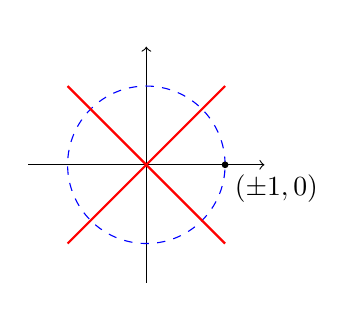
\begin{tikzpicture}[scale=0.5]
% Left diagram: Circle with lines through origin
\draw[->] (-3,0) -- (3,0) node[right]{};
\draw[->] (0,-3) -- (0,3) node[above]{};
\draw[dashed, blue] (0,0) circle (2cm);
\draw[thick, red] (0,0) -- (2,2);
\draw[thick, red] (0,0) -- (-2,2);
\draw[thick, red] (0,0) -- (2,-2);
\draw[thick, red] (0,0) -- (-2,-2);
\filldraw (2,0) circle (2pt) node[below right]{$(\pm 1, 0)$};
\end{tikzpicture}
\end{center}

This identification yields a space equivalent to the following:

\begin{center}
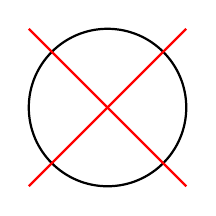
\begin{tikzpicture}[scale=0.5]
% Right diagram: Circle with a point identified
\draw[thick] (0,0) circle (2cm);
\draw[thick, red] (0,0) -- (2,2);
\draw[thick, red] (0,0) -- (-2,2);
\draw[thick, red] (0,0) -- (2,-2);
\draw[thick, red] (0,0) -- (-2,-2);
\end{tikzpicture}
\quad \equiv \quad
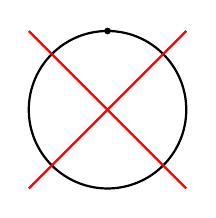
\begin{tikzpicture}[scale=0.5]
% Right diagram: Circle with a single point
\draw[thick] (0,0) circle (2cm);
\draw[thick, red] (0,0) -- (2,2);
\draw[thick, red] (0,0) -- (-2,2);
\draw[thick, red] (0,0) -- (2,-2);
\draw[thick, red] (0,0) -- (-2,-2);
\filldraw (0,2) circle (2pt);
\end{tikzpicture}
\end{center}

(Look at \textbf{Quotient Topology})
\end{remark}

% --- Page 22 ---
The content in the image does not explicitly contain any theorem, lemma, proposition, or corollary statements with proofs or formal headings. It primarily consists of definitions and explanations related to the space of lines in \(\mathbb{R}^3\) and the real projective space.


---

\begin{definition}\label{def:space_of_lines}
The space of lines in \(\mathbb{R}^3\) can be visualized as follows:

\[
\begin{tikzpicture}[scale=0.5]
    % This is a conceptual illustration, not actual TikZ code
    % The image shows a sphere with a line through the origin and a point on the sphere.
    % The right side shows a topological space resembling a sphere with a point attached.
\end{tikzpicture}
\]

The space of lines through the origin in \(\mathbb{R}^3\) is topologically equivalent to the space depicted on the right.
\end{definition}

\begin{definition}\label{def:real_projective_space}
The real projective space of dimension \(n\), denoted by \(\mathbb{R}P^n\), is the space of lines passing through the origin in \(\mathbb{R}^{n+1}\).

\[
\mathbb{R}P^n = \frac{\mathbb{R}^{n+1} \setminus \{0\}}{\sim}
\]

where \((v = \lambda v', \lambda \neq 0)\) defines the equivalence relation \(\sim\).

This can be expressed as:

\[
\mathbb{R}P^n = \left\{ [\alpha_1, \alpha_2, \ldots, \alpha_{n+1}] \mid \text{at least one } \alpha_i \text{ is non-zero} \right\}
\]

Here, \([\alpha_1, \alpha_2, \ldots, \alpha_{n+1}]\) represents the line passing through \((\alpha_1, \ldots, \alpha_{n+1})\).

Observe that \([\alpha_1, \alpha_2, \ldots, \alpha_{n+1}] = [\lambda \alpha_1, \lambda \alpha_2, \ldots, \lambda \alpha_{n+1}]\) if there is \(\lambda \neq 0\) such that \(\alpha_i = \lambda y_i\) for each \(i = 1, \ldots, n+1\).
\end{definition}

% --- Page 23 ---
Exercise: $\mathbb{R}P^2$ is not homeomorphic to $S^2$.

\begin{definition}\label{def:orientable}
A manifold is \underline{orientable} if it admits a consistent choice of orientation across its entire surface.
\end{definition}

\begin{theorem}\label{thm:nonorientable}
$\mathbb{R}P^2$ is non-orientable.
\end{theorem}

\begin{theorem}\label{thm:orientable}
$S^2$ is orientable.
\end{theorem}

\begin{theorem}\label{thm:homeomorphism}
$\mathbb{R}P^3 \cong SO(3)$ (i.e., homeomorphism).
\end{theorem}

\begin{definition}\label{def:rp3}
$\mathbb{R}P^3 = \frac{\mathbb{R}^4 \setminus \{0\}}{\sim}$ where $\mathbf{v} \sim \lambda \mathbf{v}$ for $\lambda \neq 0$.
\end{definition}

\[
\mathbb{R}P^3 = \left\{ [x_1, x_2, x_3, x_4] \mid \text{at least one } x_i \neq 0 \right\}
\]

\begin{definition}\label{def:so3}
$SO_3(\mathbb{R}) = \left\{ \text{All 3-dimensional orthogonal matrices with determinant } = 1 \right\}$
\end{definition}

\[
SO_3(\mathbb{R}) = \left\{ \text{All rotation matrices in } \mathbb{R}^3 \right\}
\]

% --- Page 24 ---
Observe that for any line passing through the origin, we can represent it by the following:

\[
[\alpha_1, \dots, \underline{\alpha_i}, \dots, \alpha_{n+1}] = \left[\frac{\alpha_1}{\alpha_i}, \dots, 1, \frac{\alpha_{i+1}}{\alpha_i}, \dots, \frac{\alpha_{n+1}}{\alpha_i}\right]
\]

We can represent a line by

\[
[y_1, y_2, \dots, 1, \dots, y_{n+1}]
\]

We will show that $\mathbb{R}P^n$ is a smooth manifold.

\[
\varphi_1 \colon \mathbb{R}P^n \to \mathbb{R}^n
\]

\[
\varphi_1 \colon \left\{ [\alpha_1, \dots, \alpha_{n+1}] \mid \alpha_1 \neq 0 \right\} \to (y_2, \dots, y_{n+1})
\]

We can form a chart in $\mathbb{R}P^1$ space.

\[
\varphi_1 \colon \left\{ [\alpha, y] \mid \alpha \neq 0 \right\} \to \text{removes } y\text{-axis}
\]

\[
\varphi_2 \colon \left\{ [\alpha, y] \mid y \neq 0 \right\} \to \text{removes } x\text{-axis}
\]

Now in $\mathbb{R}P^n$ we can define

\[
\varphi_i \colon \left\{ [\alpha_1, \dots, \underline{\alpha_i}, \dots, \alpha_{n+1}] \mid \alpha_i \neq 0 \right\} \to \mathbb{R}^n
\]

\[
[\alpha_1, \dots, \alpha_{n+1}] \mapsto \left(\frac{\alpha_1}{\alpha_i}, \dots, \frac{\alpha_{i-1}}{\alpha_i}, \frac{\alpha_{i+1}}{\alpha_i}, \dots, \frac{\alpha_{n+1}}{\alpha_i}\right)
\]

\begin{claim}
The collection of the above charts forms an atlas. (Prove): We have to show compatibility.
\end{claim}

% --- Page 25 ---
\begin{itemize}
    \item The domains have a non-empty intersection.
    \item Both are differentiable, invertible maps and as we work in finite dimension, $\varphi_i$ will have a continuous inverse. Hence, all $\varphi_i$ are compatible. (\checkmark)
\end{itemize}

In the case of $\mathbb{RP}^2$,

\begin{definition}\label{def:differentiable_map_rp}
    $\varphi_2 \circ \varphi_1^{-1} : \mathbb{R}^n \to \mathbb{R}^n$ is differentiable map in the usual sense.
\end{definition}

\begin{definition}\label{def:rp_n}
    $\mathbb{RP}^n = S^n / \sim$ where $a \sim b$ if $a = b$ or $a = -x$, $b = -x$ or $a = -x$, $b = x$.
\end{definition}

% --- Page 26 ---
---

\begin{definition}\label{def:smooth_function}
Let $X$ be a smooth manifold and $X$ has an atlas $\mathcal{A}$.

\begin{enumerate}
    \item Let $f: X \to \mathbb{R}$ be $f^n$. Let $x_0 \in X$ be a point. We say $f$ is differentiable at $x_0$ if for any chart $(U, \varphi)$ containing $x_0$, the function $f \circ \varphi^{-1} : \varphi(U) \to \mathbb{R}$ is differentiable (smooth) at $\varphi(x_0)$.

    \item Let $(a, b)$ denote an open interval in $\mathbb{R}$. We say that $g: (a, b) \to X$ is differentiable if for a chart $(V, \psi)$, the function $\psi \circ g : (a, b) \to \mathbb{R}^n$ is differentiable at all points in $(a, b)$.
\end{enumerate}
\end{definition}

---

% --- Page 27 ---
\begin{definition}\label{def:differentiability_function}
Using \cref{def:1}, we can define differentiability of function
\[ g \colon X \to \mathbb{R}^m. \]
We say that $g \colon X \to \mathbb{R}^m$ is differentiable (diff.)
if each component of $g$, say $g_i \colon X \to \mathbb{R}$,
\[ (g_i \circ \pi_i \circ g) \text{ is differentiable.} \]

Say $g = (g_1, \dots, g_m)$.
\end{definition}

\begin{definition}\label{def:smooth_map_manifolds}
In general, $X \to Y$ is smooth manifold and
$f \colon X \to Y$ be a function. We say that $f$ is differentiable (diff.) or smooth
if any chart $(U, \varphi)$ and $(V, \psi)$, where $(U, \varphi)$
is a chart for $X$, and $(V, \psi)$ is a chart for $Y$,
\[ \psi \circ f \circ \varphi^{-1} \colon \varphi(U \cap f^{-1}(V)) \to \psi(V) \]
is differentiable and check $\operatorname{Im} f \cap V \neq \emptyset$.
\end{definition}

% --- Page 28 ---
\begin{example}\label{ex:manifold_examples}

\begin{enumerate}
    \item Euclidean space $\mathbb{R}^n$ is a manifold, with an atlas of one chart.

    \item The 2-sphere $S^2$ is defined as
    \[
    S^2 = \left\{ (x,y,z) \mid x^2 + y^2 + z^2 = 1 \right\}.
    \]
    It can be covered by two charts $\varphi_1$ and $\varphi_2$ as depicted below:

    \begin{center}
    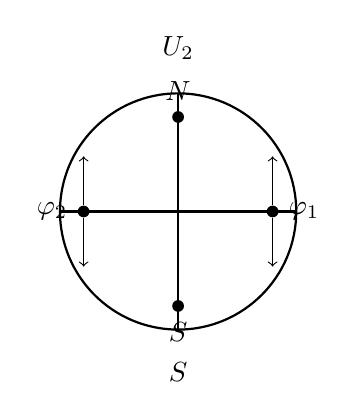
\begin{tikzpicture}[baseline=(current bounding box.center)]
        \draw[thick] (0,0) circle (1.5cm);
        \draw[thick] (-1.5,0) -- (1.5,0);
        \draw[thick] (0,-1.5) -- (0,1.5);
        \draw[thick,dashed] (0,0) -- (0,1.5);
        \draw[thick,dashed] (0,0) -- (1.5,0);
        \node[circle,fill,inner sep=1.5pt,label=above:{$N$}] (N) at (0,1.2) {};
        \node[circle,fill,inner sep=1.5pt,label=below:{$S$}] (S) at (0,-1.2) {};
        \node[circle,fill,inner sep=1.5pt,label=right:{$\varphi_1$}] (phi1) at (1.2,0) {};
        \node[circle,fill,inner sep=1.5pt,label=left:{$\varphi_2$}] (phi2) at (-1.2,0) {};
        \draw[->] (phi1) -- (1.2,0.7);
        \draw[->] (phi2) -- (-1.2,0.7);
        \draw[->] (phi1) -- (1.2,-0.7);
        \draw[->] (phi2) -- (-1.2,-0.7);
        \node[above] at (0,1.8) {$U_2$};
        \node[below] at (0,-1.8) {$S$};
    \end{tikzpicture}
    \end{center}
\end{enumerate}
\end{example}

% --- Page 29 ---
3.
For a planar pendulum, the configuration space is given by the map
\[
\varphi \colon \mathbb{R} \to S^1, \quad t \mapsto (\cos t, \sin t)
\]
with charts \(U_1 = (-\pi, \pi)\) and \(U_2 = (0, 2\pi)\).

4.
\begin{enumerate}
    \item Double Pendulum \(\Rightarrow T^2 = S^1 \times S^1\)
    \item Spherical Pendulum \(\Rightarrow S^2\)
    \item Double Spherical Pendulum \(\Rightarrow S^2 \times S^2\)
\end{enumerate}

5.
We get coordinate system
\[
\mathbb{R}^2 \times S^1
\]
for a line in the plane.

\begin{center}
    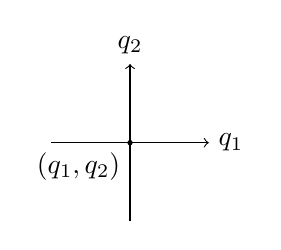
\begin{tikzpicture}[scale=0.5]
        \draw[->] (-2,0) -- (2,0) node[right]{$q_1$};
        \draw[->] (0,-2) -- (0,2) node[above]{$q_2$};
        \draw[fill=black] (0,0) circle (1.5pt) node[below left]{$(q_1,q_2)$};
    \end{tikzpicture}
\end{center}

6.
Given: Rigid Right \(\triangle OAB\) moves around \(O\) and is given by vector \(OA \in S^2\) and \(OB \in S^1\) will be a vector on the plane \(\perp^{ev}\) to \(OA\).

\begin{center}
    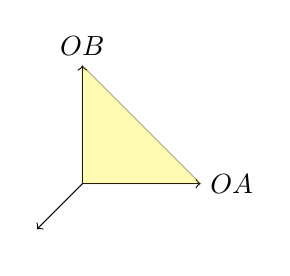
\begin{tikzpicture}[scale=0.5]
        \draw[->] (0,0,0) -- (3,0,0) node[right]{$OA$};
        \draw[->] (0,0,0) -- (0,3,0) node[above]{$OB$};
        \draw[->] (0,0,0) -- (0,0,3) node[below]{};
        \draw[fill=yellow,opacity=0.3] (0,0,0) -- (3,0,0) -- (0,3,0) -- cycle;
    \end{tikzpicture}
\end{center}

% --- Page 30 ---
The three vectors we get are
\[
\mathbf{e}_1 = \frac{OA}{|OA|}, \quad \mathbf{e}_2 = \frac{OB}{|OB|},
\]
and $\mathbf{e}_3 = \mathbf{e}_1 \times \mathbf{e}_2$. Equivalently, to
\[
M = \begin{pmatrix}
1 & 1 & 1 \\
\mathbf{e}_1 & \mathbf{e}_2 & \mathbf{e}_3
\end{pmatrix}
\]
with $\det M = 1$.

\begin{problem}
SO(3) is homeomorphic to $\mathbb{RP}^2$.
\end{problem}

\begin{definition}\label{def:degree_freedom}
The dimension of the configuration space is $\leq$ degree of freedom.
\end{definition}

\begin{definition}\label{def:embedded_manifolds}
What are embedded manifolds? How to show every manifold can be embedded in a Euclidean space?
\end{definition}

Let $X$ be a smooth manifold and $p$ be a point in $X$. The tangent space to $X$ at $p$ is of dimension $n$.

There is a chart for $X$, say $(U, \varphi)$, containing point $p$. Assume $p = (0, \ldots, 0)$ (an $n$-tuple).

% --- Page 31 ---
---

\begin{definition}\label{def:tangent_vectors}
Tangent vectors at a point $p$ as velocity vectors.
\end{definition}

We obtain curves passing through point $p$ by taking inverse images of straight line segments under $\varphi$. That is, we get curves
\[
r_v(t) = \varphi^{-1}(ct \cdot v),
\]
where $t \in (-\varepsilon, \varepsilon)$ and $r_v(0) = \varphi^{-1}(0) = p$.
\end{proof}

---

% --- Page 32 ---
We say that two locally defined curves $\gamma_1$ and $\gamma_2$ through $p$ (i.e., $\gamma_1(0) = \gamma_2(0) = p$) are \textbf{equivalent} for any chart if

\[
\left.\frac{d}{dt} (\varphi \circ \gamma_1)\right|_{t=0} = \left.\frac{d}{dt} (\varphi \circ \gamma_2)\right|_{t=0}.
\]

\begin{definition}\label{def:equivalent_curves}
Two locally defined curves $\gamma_1$ and $\gamma_2$ through $p$ are called \textbf{equivalent} if for any chart $\varphi$ around $p$,

\[
\left.\frac{d}{dt} (\varphi \circ \gamma_1)\right|_{t=0} = \left.\frac{d}{dt} (\varphi \circ \gamma_2)\right|_{t=0}.
\]
\end{definition}

\begin{remark}\label{rem:equivalence_relation}
Observe that this can construct an equivalence relation on the set of curves that pass through $p$.
\end{remark}

\begin{remark}\label{rem:independence_chart}
The independence of the definition of the choice of chart is given by

\[
\left.\frac{d}{dt} (\varphi \circ \gamma_1)\right|_{t=0} = \left.\frac{d}{dt} (\varphi \circ \gamma_2)\right|_{t=0}
\]

implies

\[
\left.\frac{d}{dt} (\psi \circ \varphi^{-1} \circ \varphi \circ \gamma_1)\right|_{t=0} = \left.\frac{d}{dt} (\psi \circ \varphi^{-1} \circ \varphi \circ \gamma_2)\right|_{t=0}.
\]

Applying the chain rule,

\[
D(\psi \circ \varphi^{-1})(\varphi \circ \gamma_1)\left.\cdot \frac{d}{dt} (\varphi \circ \gamma_1)\right|_{t=0} = D(\psi \circ \varphi^{-1})(\varphi \circ \gamma_2)\left.\cdot \frac{d}{dt} (\varphi \circ \gamma_2)\right|_{t=0}.
\]
\end{remark}

% --- Page 33 ---
As $\varphi_0 r_1(0) = \varphi_0 r_2(0) = 0$, we get,
\[
D(\varphi_0 \varphi^{-1}) \cdot \frac{d}{dt} (\varphi_0 r_1) = D(\varphi_0 \varphi^{-1}) \cdot \frac{d}{dt} (\varphi_0 r_1)
\]

\begin{definition}\label{def:tangent_vector}
A \underline{tangent vector} to $X$ at $p$ is an equivalence class of curves that pass through $p$.
\end{definition}

\begin{remark}\label{rem:computational_purpose}
For computational purposes, consider the straight line segment in a chart.
\end{remark}

\begin{definition}\label{def:tangent_space}
The set of all tangent vectors at $p$ is called a \underline{tangent space} to $X$ at $p$. Denoted by $T_p X$.
\end{definition}

\begin{definition}\label{def:local_coordinate_tangent}
In a local coordinate system, if $x \in T_p X$, then
\[
x = \sum_{i=1}^n c_i \frac{\partial}{\partial x_i}
\]
where $\frac{\partial}{\partial x_i}$ denotes the tangent vector along the $i$th coordinate of the chart.
\end{definition}

% --- Page 34 ---
\textbf{Tangent vector as derivations}

\textbf{Recall}

If $V$ is a vector space over $\mathbb{R}$ then we have $T: V \to \mathbb{R}$ linear functional.

Observe, $V^* = \{T: V \to \mathbb{R}\}$ is a vector space.

Consider $C^\infty(\mathbb{R}^n) = \{f \mid f: \mathbb{R}^n \to \mathbb{R}, f \text{ is smooth}\}$.

\begin{exercise}
$C^\infty(\mathbb{R}^n)$ is a vector space over $\mathbb{R}$. (Note: hard check)
\end{exercise}

\begin{remark}
$C^\infty(\mathbb{R}^n)$ is more than a vector space, if $f, g \in C^\infty(\mathbb{R}^n)$ then $f(x)g(x)$. This is an algebra.
\end{remark}

\begin{definition}\label{def:derivation}
A \underline{derivation} on $C^\infty(\mathbb{R}^n)$ is a linear function
\[
v: C^\infty(\mathbb{R}^n) \to \mathbb{R}
\]
such that
\[
v(fg) = v(f)g + f v(g) \quad \text{(Leibniz Rule)}
\]
\end{definition}

\begin{example}\label{ex:partial_derivative}
\[
v = \frac{\partial}{\partial x_i} \bigg|_a \quad \text{where } a \in \mathbb{R}^n
\]
\end{example}

\begin{example}\label{ex:verify_derivation}
Verify that $v$ is a derivation.

\[
\frac{\partial}{\partial x_i} \bigg|_a \text{ is a linear function } v: C^\infty(\mathbb{R}^n) \to \mathbb{R}
\]
and
\[
v(fg) = v(f)g + f v(g)
\]
\end{example}

% --- Page 35 ---
\begin{itemize}
    \item[]
    \[
    \frac{\partial}{\partial x_i} \bigg|_a (cf) = c \frac{\partial f}{\partial x_i} \bigg|_a
    \]

    \item[]
    \[
    \frac{\partial}{\partial x_i} \bigg|_a (f + g) = \frac{\partial f}{\partial x_i} \bigg|_a + \frac{\partial g}{\partial x_i} \bigg|_a
    \]

    \item[]
    \[
    \frac{\partial}{\partial x_i} \bigg|_a (cf) = c \frac{\partial f}{\partial x_i} \bigg|_a
    \]

    \item[]
    \[
    \frac{\partial}{\partial x_i} \bigg|_a (fg) = f(ca) \frac{\partial g}{\partial x_i} \bigg|_a + \frac{\partial f}{\partial x_i} \bigg|_a g(ca)
    \]

    \item[]
    If $u$ is a vector in $\mathbb{R}^n$, then the directional derivatives
    \[
    D_u : C^\infty(\mathbb{R}^n) \to \mathbb{R}
    \]
    \[
    D_u (f) \bigg|_a = D_u f = \langle \nabla f \big|_a, u \rangle
    \]
\end{itemize}

% --- Page 36 ---
Exercise:

\begin{enumerate}
    \item \textbf{Set of all derivations forms a vector space}

    \item \textbf{Show that the set $\left\{ \frac{\partial}{\partial x_1}, \frac{\partial}{\partial x_2}, \ldots, \frac{\partial}{\partial x_n} \right\}$ forms a basis for $\mathcal{D}(\mathbb{R}^n)$}

    \begin{definition}
        \label{def:derivation_basis}
        For $v \in \mathcal{D}(\mathbb{R}^n)$,
        \[
        v = \sum_{i=1}^n c_i \frac{\partial}{\partial x_i}, \quad \text{where } c_i \in \mathbb{R}.
        \]
    \end{definition}

    \begin{proof}
        Set $c_j := v(\pi_j)$, where $\pi_j$ is the projection onto the $j$-th coordinate.

        For $f \in C^\infty(\mathbb{R}^n)$,
        \[
        v(f) := \left( \sum_{i=1}^n c_i \frac{\partial}{\partial x_i} \right) (f).
        \]

        Observe that
        \[
        \left\{ \frac{\partial}{\partial x_i} \right\}_{i=1}^n
        \]
        is a linearly independent set of size $n$.

        \begin{remark}
            \label{rem:basis_size}
            Since it is a linearly independent set of size $n$, it is a basis of the space of derivations.
        \end{remark}
    \end{proof}
\end{enumerate}

% --- Page 37 ---
Let $v$ denote a tangent vector (an equivalence class of curves through $p$). In particular, $v = [\gamma]$, where $\gamma$ is a representative of $v$. We can think of $v$ as a derivation as follows:

\[
v : C^\infty(\mathbb{R}^n) \to \mathbb{R}, \quad v(f) = \frac{d}{dt}(f \circ \gamma)\Big|_{t=0}.
\]

\begin{exercise}
Show $v$ gives a well-defined derivation.
\end{exercise}

\begin{proof}
If $v = [\gamma_1] = [\gamma_2]$, then $\frac{d\gamma_1}{dt}\Big|_{t=0} = \frac{d\gamma_2}{dt}\Big|_{t=0}$.

\[
\frac{d(f \circ \gamma_1)}{dt}\Big|_{t=0} = \frac{d(f \circ \gamma_2)}{dt}\Big|_{t=0}.
\]

By the chain rule,

\[
Df|_{\gamma_1(0)} \circ \frac{d\gamma_1}{dt}\Big|_{t=0} = Df|_{\gamma_2(0)} \circ \frac{d\gamma_2}{dt}\Big|_{t=0}.
\]

% --- Page 38 ---
Let $M$ be a smooth manifold of dimension $n$.

The \textbf{tangent bundle} is given by
\[
TM = \bigcup_{p \in M} T_p M = \{(p, v) \mid v \in T_p M \text{ and } p \in M\}.
\]

\begin{definition}\label{def:tangent_bundle_atlas}
Claim: $TM$ is a smooth manifold, it admits an atlas $\{(V_i, \varphi_i)\}_{i \in I}$, we give an atlas on $TM$.
\end{definition}

\begin{proof}
Consider a point $p \in M$ and a chart $(U, \varphi)$ around $p$ on $M$ with $\varphi(p) = 0$. The tangent space $T_p M$ is spanned by
\[
T_p M = \left\langle \left. \frac{\partial}{\partial x_1} \right|_p, \left. \frac{\partial}{\partial x_2} \right|_p, \dots, \left. \frac{\partial}{\partial x_n} \right|_p \right\rangle.
\]

Every $v \in T_p M$ has a unique representation by $(v_1, v_2, \dots, v_n)$ where
\[
v = \sum_{i=1}^n v_i \left. \frac{\partial}{\partial x_i} \right|_p.
\]

Thus, the coordinates $(x_1, \dots, x_n, v_1, \dots, v_n)$ represent $(p, v)$.
\end{proof}

% --- Page 39 ---
---

Thus, we define a chart as follows:

\begin{definition}\label{def:chart}
Let $V_i = \{(p,v) \mid v \in T_p M \text{ and } p \in V_i\}$.

Define the map
\[
\Psi_i \colon V_i \to \mathbb{R}^n \times \mathbb{R}^n \cong \mathbb{R}^{2n},
\]
where
\[
\Psi_i(p,v) = (\varphi(p), v_1, v_2, \dots, v_n).
\]
The differential of $\varphi$ is given by
\[
d\varphi(v) = \sum_{i=1}^n v_i \frac{\partial}{\partial x_i} \bigg|_{\varphi(p)}.
\]
\end{definition}

To verify the claim, we need to check the following:

\begin{enumerate}
    \item $TM = \bigcup_i V_i$ (Exercise).

    \item The transition functions are smooth.
\end{enumerate}

\begin{remark}\label{rem:transition}
Observe $\Psi_i \circ \Psi_j^{-1}$:
\[
\Psi_j(V_i \cap V_j) \xrightarrow{\Psi_i \circ \Psi_j^{-1}} \Psi_i(V_i \cap V_j).
\]
\end{remark}

---

% --- Page 40 ---
---
\[
\varphi_{j} \circ \varphi_{i}^{-1} \left[ (\alpha, u) \right] = \left( \varphi_{j} \circ \varphi_{i}^{-1} (\alpha), \, d(\varphi_{j} \circ \varphi_{i}^{-1})(u) \right)
\]

\[
d(\varphi_{j} \circ \varphi_{i}^{-1})
\]

\begin{definition}\label{def:transition_map}
The above composition is smooth. Note the vector
\[
\alpha \in T_{\alpha} \mathbb{R}^{2n}
\]
is by applying the Jacobian of $\varphi_{j} \circ \varphi_{i}^{-1}$ at $\alpha$.
\end{definition}
---

% --- Page 41 ---
\begin{example}\label{ex:tangent_bundle}
\begin{enumerate}
    \item $T\mathbb{R}^n = \{(cp, v) \mid v \in T_p \mathbb{R}^n, p \in \mathbb{R}^n \} = \mathbb{R}^n \times \mathbb{R}^n$

    \item $M = S^1$, $TM = \{(cp, v) \mid v \in T_p S^1, p \in S^1 \} \cong S^1 \times \mathbb{R}$ (Diffeomorphic) (Lie Group).

    \item $M = S^2$, $TM = \{(cp, v) \mid p \in S^2, v \in T_p S^2 \}$.
    Guess: $TS^2 \cong S^2 \times \mathbb{R}^2$ is NOT true.
\end{enumerate}
\end{example}

Consider the map $\pi: TM \to M$ defined by
\[
\pi(p, v) \mapsto p.
\]

\begin{claim}\label{clm:pi_smooth}
$\pi$ is a smooth map. $\forall \varphi, \varphi^{-1}$ is differentiable.
\end{claim}

\begin{proof}
(Verify the claim)
\end{proof}

\begin{definition}\label{def:differential_map}
Suppose $M$ and $N$ are two smooth manifolds and $\varphi: M \to N$ is a smooth map.
\[
D\varphi(p, v) = (\varphi(p), d\varphi(v)).
\]
\end{definition}

\begin{remark}\label{rem:differential_properties}
The map $D\varphi$ is smooth and linear when restricted to each tangent space.
\end{remark}

% --- Page 42 ---
\begin{definition}\label{def:vector_field}
A \textbf{vector field} is a smooth function $s: M \to TM$ such that $\pi \circ s = \mathrm{id}_M$.
\end{definition}

\begin{definition}\label{def:flow_generated}
The \textbf{flow generated by a vector field} $X$ is a smooth 1-parameter family $\phi_t: M \to M$ with $\phi_0 = \mathrm{id}_M$ and is called the flow generated by vector field $X$ on $M$.
\end{definition}

\begin{remark}\label{rem:flow_existence}
\textbf{Fact:} Each vector field on a compact manifold admits a flow.
\end{remark}

\begin{example}\label{ex:vector_field_s2}
Consider the vector field $X: S^2 \to TS^2$ defined by
\[
X = \{(p, v) \mid \|p\| = 1, \langle p, v \rangle = 0\}
\]
where $S^2 \subset \mathbb{R}^3 \times \mathbb{R}^3$.

Let $P = \{(x, y, z) \mid x^2 + y^2 + z^2 = 1\}$ and $Q = \{(u, v, w) \mid \langle (x, y, z), (u, v, w) \rangle = 0\}$.
Then $P \cap Q$ is 1-dimensional.

Take the unit vector in $P \cap Q$ based at $(x_0, y_0, z_0)$. Scale it by a factor $(1 - z_0)(1 + z_0)$.
\end{example}

% --- Page 43 ---
---

\begin{example}\label{ex:cotangent_bundle}
\textbf{1-forms and co-tangent bundles}

On $(\mathbb{R}^n, (x_1, \dots, x_n))$ we have $d x_i \colon \mathbb{R}^n \to \mathbb{R}$ linear maps
\[
d x_i (v) = c_i \quad \text{where} \quad v = \sum_{i=1}^n c_i e_i,
\]
where $e_i = (0, \dots, 1, \dots, 0)$ (1 in the $i^{\text{th}}$ place).
\end{example}

\begin{proof}
\textbf{Exercise:} Verify $d x_i$ is a linear map. (Trivial)
\end{proof}

By definition $d x_i \in (\mathbb{R}^n)^* = \{ f \colon \mathbb{R}^n \to \mathbb{R} \mid f \text{ is linear} \}$.

Note that $(\mathbb{R}^n)^*$ is a vector space of dimension $n$ with a basis
\[
\{ d x_1, \dots, d x_n \}.
\]

We can repeat the above argument for each tangent space $p \in \mathbb{R}^n$:
\[
T_p \mathbb{R}^n = \left\langle \left. \frac{\partial}{\partial x_1} \right|_p, \dots, \left. \frac{\partial}{\partial x_n} \right|_p \right\rangle.
\]

We consider the dual space $(T_p \mathbb{R}^n)^*$.

% --- Page 44 ---
\begin{definition}\label{def:cotangent_space}
The $(T_p \mathbb{R}^n)^*$ is the \underline{cotangent space} at $p$ (or the space of co-vectors).
\end{definition}

Thus, we have $dx_i^j : T_p \mathbb{R}^n \to \mathbb{R}$,
\[
v = \sum_{j=1}^n c_j \frac{\partial}{\partial x_j} \bigg|_p \quad \longmapsto \quad c_i.
\]

When we drop reference to point $p$, we get a family of functionals on the corresponding tangent space,
\[
dx_i : T_p \mathbb{R}^n \to \mathbb{R}.
\]

When we drop reference to point $p$, we get a family of functionals on corresponding tangent space,
\[
dx_i : \mathcal{X}(\mathbb{R}^n) \to C^\infty(\mathbb{R}^n).
\]

\begin{remark}\label{rem:smooth_vector_fields}
The space of smooth vector fields.
\end{remark}

For $v \in \mathcal{X}(\mathbb{R}^n)$, we have
\[
dx_i(v) = f(p) = c_i.
\]

$dx_i$ is a linear map from $\mathcal{X}(\mathbb{R}^n)$ to $C^\infty(\mathbb{R}^n)$.

% --- Page 45 ---
If we have a smooth function \( f \in C^\infty(\mathbb{R}^n) \) and vector field \( v \in \mathfrak{X}(\mathbb{R}^n) \), the function-valued vector field \( f v \) is a smooth vector field given by
\[
(f v)(p) = f(p) \cdot v(p).
\]

\begin{definition}\label{def:module_structure}
The space \(\mathfrak{X}(\mathbb{R}^n)\) is a module over \( C^\infty(\mathbb{R}^n) \).
\end{definition}

% --- Page 46 ---
\begin{definition}\label{def:cotangent_bundle}
Let $X$ be a smooth manifold of dimension $n$. The cotangent bundle of $X$, as a set, is given by
\[ T^*X = \bigcup_{p \in X} (T_p X)^* = \{(p, v) \mid p \in X, v \in (T_p X)^*\}. \]

In the case of $\mathbb{R}^n$,
\[ T\mathbb{R}^n = \bigcup_{p \in \mathbb{R}^n} (T_p \mathbb{R}^n). \]
\end{definition}

Suppose $(\alpha_1, \dots, \alpha_n)$ is a coordinate system on $\mathbb{R}^n$. Then,
\[ T\mathbb{R}^n = \{(p, v) \mid p \in \mathbb{R}^n, v \in (T_p \mathbb{R}^n)\} \]
\[ = \{(x_1, \dots, x_n, c_1, \dots, c_n) \mid v = \sum_{j=1}^n c_j \, d\alpha_j\}. \]

This is isomorphic to $\mathbb{R}^n \times \mathbb{R}^n$ (bundle isomorphism).
\end{definition}

\begin{remark}\label{rem:dimension_cotangent_bundle}
Claim: $T^*X$ is a smooth manifold of dimension $2n$.
\end{remark}

\begin{exercise}\label{ex:atlas_cotangent_bundle}
Exercise: Set up an atlas for $T^*X$.
\end{exercise}

\begin{proof}[Check]
Consider a chart on $T^*X$:
\[ \varphi_\alpha \colon T^*X \to \mathbb{R}^{2n}, \]
\[ (p, \xi) \mapsto (\varphi(p), \xi(\frac{\partial}{\partial x_1}), \dots, \xi(\frac{\partial}{\partial x_n})), \]
where
\[ \xi = \sum_{i=1}^n \xi_i \, d\alpha_i \quad \text{and} \quad \xi_i \in \mathbb{R}, \quad 1 \leq i \leq n. \]
\end{proof}

% --- Page 47 ---
---

Refer to chapter 7 of Arnold's book for 2 classes.

Let $X$ be a smooth manifold of dimension $n$. Then, the cotangent bundle
\[
T^*X = \bigcup_{p \in X} (T_p X)^*
\]
is a smooth manifold of dimension $2n$.

\[
T^*X = \{(p, v) \mid v \in (T_p X)^*, p \in X\}.
\]

\begin{example}\label{ex:cotangent_bundle_examples}
\begin{enumerate}
    \item $T^* \mathbb{R}^n = \mathbb{R}^n \times (\mathbb{R}^n)^*$
    \item $T^* S^1 = \{(p, v) \mid v \in (T_p S^1)^*, p \in S^1\}$
\end{enumerate}
\end{example}

Consider $T_p S^1 = \{\alpha : T_p S^1 \to \mathbb{R}\}$ with $v \mapsto \alpha(v)$.

By the Riesz Representation Theorem, each $\alpha \in (T_p S^1)^*$ corresponds to a unique vector $w$ such that
\[
\alpha(v) = \langle w, v \rangle, \quad w = \lambda e.
\]

\[
\alpha : V^* \to \mathbb{R}, \quad v \mapsto \alpha(v) = \langle w, v \rangle
\]

\[
\exists! \, w \in V \text{ such that } \alpha(v) = \lambda \langle e, v \rangle = \lambda \|v\|.
\]

\[
\implies \lambda = \frac{\alpha(v)}{\|v\|}.
\]

---

% --- Page 48 ---
A 1-form on $X$ is a smooth section of the cotangent bundle $T^*X$.

\[
T^*X = \bigsqcup_{(p,\alpha)} \mid \alpha \in (T_pX)^*, p \in X \big\}
\]

Therefore for any 1-form $\beta$, we have $\pi \circ \beta = \mathrm{id}_X$. In other words, $\beta$ is a smooth assignment of covectors to points in $X$.

\begin{example}\label{ex:cotangent_bundle_example}
    \begin{enumerate}
        \item Let $X = \mathbb{R}$, then $T^*\mathbb{R} \cong \mathbb{R} \times \mathbb{R}$,
        \[
        T^*\mathbb{R} = \bigsqcup_{(x,\alpha)} \mid \alpha \in (T_x\mathbb{R})^*, x \in \mathbb{R} \big\}.
        \]
        Define $\beta : \mathbb{R} \to T^*\mathbb{R}$ by
        \[
        x \mapsto (x, d x),
        \]
        where
        \[
        d x = \begin{cases}
        \alpha & \text{if } x = 0, \\
        0 & \text{otherwise}.
        \end{cases}
        \]
    \end{enumerate}
\end{example}

% --- Page 49 ---
Take $B_1 \colon \mathbb{R} \to T^*\mathbb{R}$ defined by
\[
x \mapsto (x, x\,da)
\]
Then $B_1$ is a $1$-form.

\begin{enumerate}
    \item For $X = \mathbb{R}^n$, to each $1$-form $B$ on $\mathbb{R}^n$, we have the following
    \[
    B(\underline{x}, \alpha_1, \dots, \alpha_n) = \sum_{i=1}^n c_i(\alpha_1, \dots, \alpha_n)\,da_i
    \]
    where $c_i$'s are smooth functions on $\mathbb{R}^n$.

    \begin{definition}\label{def:1-form}
        \[
        B \colon \mathbb{R}^n \to (T^*\mathbb{R}^n)
        \]
        \[
        x \mapsto \left(x, \sum_{i=1}^n c_i(x)\,da_i\right)
        \]
    \end{definition}

    \item Verify that $B$ is a $1$-form
    \[
    B \colon \mathbb{R}^3 \to T^*\mathbb{R}^3
    \]
    \[
    (x, y, z) \mapsto (x, y, z, dz - y\,dx)
    \]

    \begin{proof}
        Check linearity.

        Do we just have to check linearity?

        $\pi \circ B = \mathrm{id}$.
    \end{proof}
\end{enumerate}

% --- Page 50 ---
\begin{enumerate}
    \item Take $X = S^1 \subset \mathbb{R}^2$,
    \[
    S^1 = \{(x,y) \mid x^2 + y^2 = 1\}.
    \]
    \begin{definition}\label{def:1form_s1}
        We define $B_{(x,y)} = x\,dy$.
    \end{definition}

    \item Take $X = S^3 \subset \mathbb{R}^4$,
    \[
    S^3 = \{x \in \mathbb{R}^4 \mid \|x\| = 1\}.
    \]
    \begin{definition}\label{def:1form_s3}
        Define $B_{(x_1, x_2, x_3, x_4)} = x_1\,dx_1 + x_2\,dx_2 + x_3\,dx_3 + x_4\,dx_4$.
    \end{definition}

    Then $B$ is a 1-form on $S^3$.

    \begin{remark}\label{rem:check_linearity}
        Do we just check linearity?
    \end{remark}

    \begin{remark}\label{rem:check_pi}
        Not really, we also check that the $\pi \circ B = \mathrm{id}_X$.
    \end{remark}
\end{enumerate}

% --- Page 51 ---
Let $(\alpha_1, \ldots, \alpha_n)$ be the coordinate system on $\mathbb{R}^n$.

\begin{definition}\label{def:exterior_2_form}
An \underline{exterior 2-form} is a bilinear map that is skew-symmetric on $\mathbb{R}^n \times \mathbb{R}^n$ and real-valued.

In particular, if $\omega$ is an exterior 2-form (or 2-form) by definition,
\[
\omega \colon \mathbb{R}^n \times \mathbb{R}^n \to \mathbb{R}
\]
$\omega$ is linear in both variables and
\[
\omega(u,v) = -\omega(v,u) \quad \text{for all } u,v \in \mathbb{R}^n.
\]
\end{definition}

\begin{example}\label{ex:determinant_2_form}
\[
\omega \colon \mathbb{R}^2 \times \mathbb{R}^2 \to \mathbb{R}
\]
\[
(u,v) \mapsto \det \begin{pmatrix} u_1 & u_2 \\ v_1 & v_2 \end{pmatrix}
\]
where $u = (u_1, u_2)$, $v = (v_1, v_2)$.

Observe $\omega(u,v)$ gives out the area of the parallelogram formed by $u, v$.
\end{example}

% --- Page 52 ---
---

**Exercise**

Let $w: \mathbb{R}^n \times \mathbb{R}^n \to \mathbb{R}$ be an exterior 2-form such that $w \equiv 0$ if $u = v$. Show that
\[ w(\lambda u, v) = \lambda w(u, v) \quad \text{where } \lambda, v \in \mathbb{R} \]
and
\[ w(u, u) = -w(u, u) \implies w(u, u) = 0 \quad \text{for any } u \in \mathbb{R}^n \text{ and } u \neq 0. \]

---

**Exercise**

Show that the following is an exterior 2-form on $\mathbb{R}^3$. Fix $v \neq 0 \in \mathbb{R}^3$. Define
\[ w(u_1, u_2) = v \cdot (u_1 \times u_2). \]

\begin{example}\label{ex:cross_product_form}
Let $d_1$ and $d_2$ be two covectors on $\mathbb{R}^4$. Then we construct the following map:
\[ s(u, v) = \begin{vmatrix}
d_1(u) & d_2(u) \\
d_1(v) & d_2(v)
\end{vmatrix}. \]
Check that $s$ is a 2-form.
\end{example}

---

% --- Page 53 ---
We denote $s = \alpha_1 \wedge \alpha_2$.

\begin{exercise}
Take any 2-form $\omega$ on $\mathbb{R}^n$, show that
\[
\omega = \sum_{i < j} c_{ij} \, dx_i \wedge dx_j
\]
for scalars $c_{ij}$. For $u, v \in T_p \mathbb{R}^n$,
\begin{proof}
\[
\omega(u, v) = \sum_{i < j} c_{ij} \, dx_i \wedge dx_j(u, v)
\]
\[
= \sum_{i < j} c_{ij} \begin{vmatrix}
dx_i(u) & dx_i(v) \\
dx_j(u) & dx_j(v)
\end{vmatrix}
= \sum_{i < j} c_{ij} \begin{vmatrix}
u_i & v_i \\
u_j & v_j
\end{vmatrix}
\]
\[
= -\sum_{i < j} c_{ij} \begin{vmatrix}
dx_i(v) & dx_i(u) \\
dx_j(v) & dx_j(u)
\end{vmatrix}
= -\omega(v, u).
\]
and linearity comes from the elements of the determinant.
\end{proof}
\end{exercise}

% --- Page 54 ---
Let $\Lambda^2(\mathbb{C} \mathbb{R}^n)$ denote the set of 2-forms on $\mathbb{R}^n$. Note that $\Lambda^2(\mathbb{C} \mathbb{R}^n)$ forms a vector space over $\mathbb{R}$.

\[
\Lambda^2(\mathbb{C} \mathbb{R}^n) = \left\{ \omega : \mathbb{R}^n \times \mathbb{R}^n \to \mathbb{R} \mid \omega \text{ is bilinear and skew-symmetric} \right\}
\]

For $\omega_1, \omega_2 \in \Lambda^2(\mathbb{C} \mathbb{R}^n)$ and $\mu \in \mathbb{R}$,
\[
(\omega_1 + \omega_2)(u, v) = \omega_1(u, v) + \omega_2(u, v)
\]
\[
\mu \cdot \omega_2(u, v) = \mu (\omega(u, v))
\]

\begin{exercise}
Show the dimension of $\Lambda^2(\mathbb{C} \mathbb{R}^n)$ is given by $\binom{n}{2}$. (Check the previous \cref{def:dimension}.)

We first show the set $\left\{ dx_i \wedge dx_j \mid i < j \right\}$ form a basis for $\Lambda^2(\mathbb{R}^n)$. (Show)

Observe $dx_i \wedge dx_i = 0$ and $dx_i \wedge dx_j = -dx_j \wedge dx_i$ and $\left\{ dx_i \right\}_{i=1}^n$ is the basis of $T^* \mathbb{R}^n$.
\end{exercise}

% --- Page 55 ---
\begin{definition}\label{def:exterior_k_form}
An \textbf{exterior $k$-form} on $\mathbb{R}^n$ is a $k$-linear map
\[
\omega \colon \underbrace{\mathbb{R}^n \times \mathbb{R}^n \times \cdots \times \mathbb{R}^n}_{k\text{-fold product}} \to \mathbb{R}
\]
that is \textbf{skew-symmetric}, i.e.,
\[
\omega(u_1, \dots, u_k) = \text{sgn}(\sigma) \, \omega(u_{\sigma(1)}, \dots, u_{\sigma(k)})
\]
where $\sigma$ is a permutation of $\{1, \dots, k\}$.
\end{definition}

\begin{example}\label{ex:determinant_k_form}
On $\mathbb{R}^k$, we have an exterior $k$-form given by
\[
\omega(u_1, \dots, u_k) = \det \begin{bmatrix}
|u_1|_1 & \cdots & |u_1|_k \\
\vdots & \ddots & \vdots \\
|u_k|_1 & \cdots & |u_k|_k
\end{bmatrix}.
\]
Note that $\omega(u_1, \dots, u_k)$ gives the $k$-dimensional volume of the parallelepiped formed by the $k$-vectors $u_1, \dots, u_k$.
\end{example}

% --- Page 56 ---
---

Refer to chapter 7 in Arnold.

\begin{definition}\label{def:wedge_product}
\textbf{Wedge product on exterior forms.}

Let $\omega^k$ and $\omega^l$ be a $k$-form, $l$-form on $\mathbb{R}^n$ respectively.

Define:
\[
\omega^k \wedge \omega^l \quad (\text{an exterior } (k+l) \text{ form on } \mathbb{R}^n)
\]

\[
(\omega^k \wedge \omega^l)(u_1, \dots, u_k, u_{k+1}, \dots, u_{k+l})
\]

\[
= \sum (-1)^\nu \omega^k(u_{i_1}, \dots, u_{i_k}) \cdot \omega^l(u_{i_{k+1}}, \dots, u_{i_{k+l}})
\]

where $i_1 < i_2 < \dots < i_{k+l}$ and $\nu = \begin{cases}
1 & \text{if the permutation is odd} \\
0 & \text{if the permutation is even}
\end{cases}$
\end{definition}

\begin{exercise}\label{ex:verify_wedge_product}
Verify that the definition gives a $(k+l)$-form.
\end{exercise}

Recall if $\omega_1$ and $\omega_2$ are $1$-forms then, we defined $(\omega_1 \wedge \omega_2)(u_1, u_2)$ as:

\[
\begin{vmatrix}
\omega_1(u_1) & \omega_1(u_2) \\
\omega_2(u_1) & \omega_2(u_2)
\end{vmatrix}
= \omega_1(u_1)\omega_2(u_2) - \omega_1(u_2)\omega_2(u_1)
\]

---

% --- Page 57 ---
---

The wedge product $\wedge$ satisfies the following properties:

\begin{enumerate}[(1)]
    \item
    \[
    w^k \wedge w^\ell = (-1)^{k\ell} w^\ell \wedge w^k
    \]

    \begin{proof}
    I am still unclear on how we consider if $k$ and $\ell$ indices are swapped, or is the argument I gave above suffice where we consider the permutation on $k\ell$.
    \end{proof}

    \item
    \[
    (w^k \wedge w^\ell) \wedge w^m = w^k \wedge (w^\ell \wedge w^m)
    \]

    \item
    \[
    (\lambda_1 w_1^k + \lambda_2 w_2^k) \wedge w^m = \lambda_1 (w_1^k \wedge w^m) + \lambda_2 (w_2^k \wedge w^m).
    \]
\end{enumerate}

\begin{exercise}
Verify the above properties hold. I can intuitively think why the above properties hold, but I am unable to write/show where the changes are happening once I express $w^k \wedge w^\ell$ into a summation (Do I even need to do that?).
\end{exercise}

---

% --- Page 58 ---
On $\mathbb{R}^{2n}$ with coordinate $(p_1, p_2, \dots, p_n, q_1, \dots, q_n)$, we define the following 2-form

\[
\omega^2 = \sum_{i=1}^n dp_i \wedge dq_i,
\]

where $\{dp_1, \dots, dp_n, dq_1, \dots, dq_n\}$ denote the dual basis.

\begin{enumerate}
    \item[(1)] Compute $\omega^2 \wedge \omega^2$

    \item[(2)] Compute $\omega^2 \wedge \omega^2 \wedge \dots \wedge \omega^2$ $k$ times $= (\omega^2)^k$

    \begin{definition}\label{def:kth_power_of_omega}
        \[
        (\omega^2)^k = k! \sum_{1 \leq i_1 < \dots < i_k \leq n} dp_{i_1} \wedge dq_{i_1} \wedge \dots \wedge dp_{i_k} \wedge dq_{i_k}
        \]
    \end{definition}
\end{enumerate}

% --- Page 59 ---
\[
\omega^2 \wedge \omega^2 = \left( \sum_{i=1}^n dp_i \wedge dq_i \right) \wedge \left( \sum_{j=1}^n dp_j \wedge dq_j \right)
\]

\[
= \left( dp_1 \wedge dq_1 + dp_2 \wedge dq_2 + \cdots + dp_n \wedge dq_n \right) \wedge \left( dp_1 \wedge dq_1 + dp_2 \wedge dq_2 + \cdots + dp_n \wedge dq_n \right)
\]

\[
= (dp_1 \wedge dq_1) \wedge (dp_1 \wedge dq_1) + (dp_1 \wedge dq_1) \wedge (dp_2 \wedge dq_2) + \cdots + (dp_n \wedge dq_n) \wedge (dp_n \wedge dq_n)
\]

\[
= (dp_1 \wedge dq_1 \wedge dp_1 \wedge dq_1) + \cdots
\]

\[
= 0 + \cdots
\]

Observe that,
\[
(dp_i \wedge dq_i) \wedge (dp_i \wedge dq_i) = 0
\]
for all \(1 \leq i \leq n\).

But, for \(i \neq j\),
\[
(dp_i \wedge dq_i) \wedge (dp_j \wedge dq_j)
\]
appears twice.

\[
\therefore \quad \omega^2 \wedge \omega^2 = 2 \sum_{i < j} dp_i \wedge dq_i \wedge dp_j \wedge dq_j
\]

% --- Page 60 ---
Given a vector $u \in \mathbb{R}^3$, we consider the 2-form
\[
\omega_u(v_1, v_2) = u \cdot (v_1 \times v_2) \quad \text{for} \quad v_1, v_2 \in \mathbb{R}^3.
\]

To find the wedge product of $\omega_{u_1}$ and $\omega_{u_2}$, we have:

\[
\omega_{u_1} \wedge \omega_{u_2}(v_1, v_2, v_3, v_4) = \sum_{\sigma \in S_4} \text{sgn}(\sigma) \, \omega_{u_1}(v_{\sigma(1)}, v_{\sigma(2)}) \, \omega_{u_2}(v_{\sigma(3)}, v_{\sigma(4)})
\]

\[
= \sum_{\sigma \in S_4} \text{sgn}(\sigma) \left( u_1 \cdot (v_{\sigma(1)} \times v_{\sigma(2)}) \right) \left( u_2 \cdot (v_{\sigma(3)} \times v_{\sigma(4)}) \right)
\]

There is no non-trivial 4-form for dimensions in $\mathbb{R}^3$, so we get zero.

% --- Page 61 ---
Let $T: \mathbb{R}^n \to \mathbb{R}^n$ be a linear transformation and $w^k$ be an exterior $k$-form on $\mathbb{R}^m$.

We define a new exterior $k$-form on $\mathbb{R}^n$ as follows:

\begin{definition}\label{def:pullback_form}
Let $T^* w^k$ be defined by
\[
T^* w^k (v_1, \ldots, v_k) = w^k (T v_1, \ldots, T v_k).
\]
This is called the \textbf{pullback form} via $T$ or the \textbf{pullback} of $w^k$ via $T$.
\end{definition}

% --- Page 62 ---
Let $f: \mathbb{R}^n \to \mathbb{R}$ be a smooth function. For a point $x \in \mathbb{R}^n$, the derivative of $f$,
\[
df_x: T_x \mathbb{R}^n \to \mathbb{R}
\]
is a linear map. The derivative is a smooth map $df: T\mathbb{R}^n \to \mathbb{R}$ such that for each point we get an external 1-form
\[
df_x: T_x \mathbb{R}^n \to \mathbb{R}.
\]

\begin{definition}\label{def:differential_1_form}
In general, we define a differential 1-form as follows. Let $M$ be a manifold of dimension $n$. Let $TM = \bigsqcup_{x \in M} T_x M$ denote the tangent bundle of $M$. A differential 1-form on $M$ is a smooth map
\[
\omega: TM \to \mathbb{R}
\]
such that for each $x \in M$, we have
\[
\omega|_{T_x M} = \omega_x: T_x M \to \mathbb{R}
\]
an external 1-form.
\end{definition}

\begin{example}\label{ex:derivative_as_1_form}
Let $f: M \to \mathbb{R}$ be a smooth function. Then $df: TM \to \mathbb{R}$ is a differential 1-form.
\end{example}

% --- Page 63 ---
\begin{theorem}\label{thm:differential_form_coordinates}
Let $(x_1, \dots, x_n)$ denote a coordinate system on $\mathbb{R}^n$. Let $\omega$ be a differential 1-form, then
\[
\omega = \sum_{i=1}^n q_i(x_1, \dots, x_n) \, dx_i
\]
where $q_i$'s are smooth real-valued functions on $\mathbb{R}^n$.
\end{theorem}

\begin{proof}
For each $x = (x_1, \dots, x_n)$, the differential form $\omega$ restricts to be an exterior 1-form on $T_x \mathbb{R}^n$. That is,
\[
\omega_x \colon T_x \mathbb{R}^n \to \mathbb{R}.
\]
We know that $\omega_x = \sum_{i=1}^n c_i \, dx_i$, where $c_i$ are scalars depending on $x$. The smoothness of $\omega$ implies that the maps
\[
x \mapsto c_i(x)
\]
are smooth.
\end{proof}

% --- Page 64 ---
\begin{corollary}\label{cor:differential_1form_coordinates}
Let $M$ be a smooth manifold of dimension $n$ and $(U,\varphi)$ be a chart. Suppose $(x_1,\dots,x_n)$ denote the coordinate system given by $(U,\varphi)$. Then a differential 1-form $\omega$ can be equipped as follows in the coordinate chart $(U,\varphi)$:

\[
\omega = \sum_{i=1}^n a_i(x_1,\dots,x_n)\,dx_i,
\]

where $a_i$'s are smooth functions defined on the chart $(U,\varphi)$.
\end{corollary}

% --- Page 65 ---
\begin{definition}\label{def:differential_2_form}
A differential 2-form on $\mathbb{R}^n$ is a smooth map
\[
\omega^2
\]
such that for each $x \in \mathbb{R}^n$, $\omega^2_x$ is an exterior 2-form on $T_x \mathbb{R}^n$.
\end{definition}

\begin{theorem}\label{thm:differential_2_form_representation}
If $\omega^2$ is a differential 2-form on $\mathbb{R}^n$, then
\[
\omega^2 = \sum_{i < j} q_{ij}(x) \, dx_i \wedge dx_j \quad \text{(*)}
\]
where $q_{ij} \colon \mathbb{R}^n \to \mathbb{R}$ are smooth functions.
\end{theorem}

\begin{example}\label{ex:area_form}
On $\mathbb{R}^2$ with $(x, y)$ coordinates, we have the area form given by $dx \wedge dy$.
\end{example}

% --- Page 66 ---
\begin{exercise}
Change the coordinates to polar coordinates described by $(r, \Theta)$ where $x^2 + y^2 = r^2$ and $\tan \Theta = \frac{y}{x}$. How does the area form look like in $(r, \Theta)$ coordinates?
\end{exercise}

We start with the relations:
\[
x^2 + y^2 = r^2, \quad \tan \Theta = \frac{y}{x}.
\]

First, we derive the differential relations:
\[
2r \, dr = 2x \, dx + 2y \, dy = 2(x \, dx + y \, dy).
\]

Next, we compute $d\Theta$:
\[
\sec^2 \Theta \, d\Theta = \frac{x \, dy - y \, dx}{x^2}.
\]

Using the identity $1 + \tan^2 \Theta = \sec^2 \Theta$, we have:
\[
(1 + \tan^2 \Theta) \, d\Theta = \frac{x \, dy - y \, dx}{x^2}.
\]

Since $\tan \Theta = \frac{y}{x}$, we get:
\[
\frac{x^2 + y^2}{x^2} \, d\Theta = \frac{x \, dy - y \, dx}{x^2}.
\]

Simplifying, we obtain:
\[
d\Theta = \frac{x \, dy - y \, dx}{x^2 + y^2}.
\]

We also have:
\[
r \, dr = x \, dx + y \, dy,
\]
and
\[
r^2 \, d\Theta = x \, dy - y \, dx.
\]

Now, consider the wedge product of $r \, dr$ and $d\Theta$:
\[
r^3 \, dr \wedge d\Theta = (x \, dx + y \, dy) \wedge (x \, dy - y \, dx).
\]

Expanding the wedge product:
\[
r^3 \, dr \wedge d\Theta = x^2 \, dx \wedge dy - y^2 \, dy \wedge dx.
\]

Since $dx \wedge dy = -dy \wedge dx$, we have:
\[
r^3 \, dr \wedge d\Theta = x^2 \, dx \wedge dy + y^2 \, dx \wedge dy = (x^2 + y^2) \, dx \wedge dy.
\]

Given that $x^2 + y^2 = r^2$, we conclude:
\[
r \, dr \wedge d\Theta = dx \wedge dy.
\]

Thus, the area form in polar coordinates $(r, \Theta)$ is:
\[
r \, dr \wedge d\Theta.
\]

% --- Page 67 ---
\begin{definition}\label{def:differential_2_form}
A differential $2$-form $\omega^2$ on $M$ is a smooth map that restricts to each $T_x M$, for each $x$, to give an exterior $2$-form. We denote it by $\omega_x$.

In a chart $(U, \varphi = (x_1, \dots, x_n))$ on $M$, $\omega^2$ expressed in $\eqref{C*}$.
\end{definition}

On $\mathbb{R}^n$ with coordinates $(x_1, \dots, x_n)$, a basis of exterior $k$-forms is given by
\[
\left\{ dx_{i_1} \wedge \cdots \wedge dx_{i_k} \mid i_1, \dots, i_k \in \{1, \dots, n\}, \quad \text{s.t.} \quad i_1 < i_2 < \cdots < i_k \right\}.
\]

For vectors $u_1, u_2, \dots, u_k \in \mathbb{R}^n$,
\[
dx_{i_1} \wedge dx_{i_2} \wedge \cdots \wedge dx_{i_k}(u_1, u_2, \dots, u_k)
= \sum_{\sigma \in S_k} \text{sgn}(\sigma) \, dx_{i_1}(u_{\sigma(1)}) \, dx_{i_2}(u_{\sigma(2)}) \cdots dx_{i_k}(u_{\sigma(k)}).
\]

% --- Page 68 ---
Suppose $(U, \varphi)$ is a chart for $M$. Let $(x_1, \dots, x_n)$ denote the coordinate system from $(U, \varphi)$.

Then,
\[
\omega^k = \sum_{1 \leq i_1 \leq i_2 \leq \dots \leq i_k \leq n} a_{i_1 i_2 \dots i_k}(x_1, \dots, x_n) \, dx_{i_1} \wedge dx_{i_2} \wedge \dots \wedge dx_{i_k},
\]
where each $a_{i_1 i_2 \dots i_k}$ is a smooth real-valued function.

% --- Page 69 ---
\textbf{Integration of forms.}

Let $\omega$ be a differential 1-form. Given a smooth curve $\gamma: [a, b] \rightarrow M$, the curve $\gamma$ is a smooth curve $\tilde{\gamma}: (a-\varepsilon, b+\varepsilon) \rightarrow M$.

For each point $x$ on $\gamma$, we have the number $\omega_x(v)$ where $v$ is the tangent vector $\dot{\gamma}(t)$ at $x$.

\[
\int_\gamma \omega = \int_a^b \omega_{\gamma(t)}(\dot{\gamma}(t)) \, dt
\]

\begin{definition}\label{def:integration_1form}
The integral of a differential 1-form $\omega$ along a smooth curve $\gamma$ is defined as
\[
\int_\gamma \omega = \int_a^b \omega_{\gamma(t)}(\dot{\gamma}(t)) \, dt.
\]
\end{definition}

\textbf{Integral of $n$-forms.}

Let $\omega^n$ denote a differential $n$-form on $\mathbb{R}^n$.

\begin{definition}\label{def:nform}
An $n$-form $\omega^n$ on $\mathbb{R}^n$ can be expressed as
\[
\omega^n = f(x_1, \ldots, x_n) \, dx_1 \wedge dx_2 \wedge \cdots \wedge dx_n,
\]
where $f: \mathbb{R}^n \rightarrow \mathbb{R}$ is a smooth function.
\end{definition}

For a point $p \in \mathbb{R}^n$,
\[
\omega^n_p = f(p) \, dx_1 \wedge dx_2 \wedge \cdots \wedge dx_n.
\]

\begin{definition}\label{def:integral_nform}
The integral of an $n$-form $\omega^n$ over a polyhedron $\Delta^n$ is given by
\[
\int_{\Delta^n} \omega^n = \int_{\Delta^n} f(x_1, \ldots, x_n) \, dx_1 \wedge dx_2 \wedge \cdots \wedge dx_n,
\]
where $\Delta^n$ is a polyhedron which is a compact and convex $n$-dimensional subset of $\mathbb{R}^n$.
\end{definition}

% --- Page 70 ---
\begin{definition}\label{def:oriented_manifold}
Let $M$ be an $n$-dimensional manifold. Assume that $M$ is \emph{oriented}. This means that we can consistently orient $n$-dimensional parallelepipeds on $M$.
\end{definition}

Let $\omega^n$ denote a differential $n$-form on $M$.

\begin{theorem}\label{thm:integration_on_compact_manifold}
If $M$ is compact, then $M$ can be broken into nicely fitting $n$-dimensional polyhedra. The integral of $\omega^n$ over $M$ is given by
\[
\int_M \omega^n = \sum_{\Delta^n \in S} \int_{\Delta^n} \omega^n,
\]
where $S$ is the finite set of $n$-dimensional polyhedra together forming the manifold $M$.
\end{theorem}

% --- Page 71 ---
---

\begin{definition}\label{def:k-form}
Let $\omega^k$ denote a differential $k$-form on a smooth manifold $M$ of dimension $n$.
\end{definition}

\begin{definition}\label{def:convex-polyhedron}
Let $\Delta^k$ denote a convex polyhedron in $\mathbb{R}^k$ (take $(k+1)$ points and consider their convex hull).
\end{definition}

\begin{definition}\label{def:k-cell}
A $k$-cell $\sigma$ in $M$ is a triple $(\Delta^k, f, \text{Or})$, where
\begin{itemize}
    \item $\Delta^k$ is a convex polyhedron in $\mathbb{R}^k$,
    \item $f \colon \Delta^k \to M$ is a smooth function,
    \item $\text{Or}$ denotes an orientation on $\Delta^k$.
\end{itemize}
\end{definition}

\begin{example}\label{ex:oriented-path}
An (oriented) path is a $1$-cell:
\[
f \colon [a,b] \to M.
\]
\end{example}

\begin{definition}\label{def:k-chain}
A $k$-chain is a formal integral combination of $k$-forms. If $\sigma_1, \sigma_2, \dots, \sigma_r$ are $k$-cells, then a $k$-chain is a formal integral combination
\[
\sum_{i=1}^r m_i \sigma_i,
\]
where $m_i \in \mathbb{Z}$.
\end{definition}

\begin{remark}\label{rem:2-cell-annulus}
Note: Each $t_i$ is a $2$-cell in the annulus.
\end{remark}

% --- Page 72 ---
Then, $T_1 + T_2 + \cdots + T_6$ is a $2$-chain in the annulus.

Another $2$-chain is $2T_1 + 4T_2 + 6T_3 + 7T_4$.

\[
C^k = \sum_{i=1}^r m_i \sigma_i \quad \text{is defined as}
\]

\[
\int_{C^k} \omega^k = \sum_{i=1}^r m_i \int_{\sigma_i} \omega^k
\]

% --- Page 73 ---
\textbf{Exterior derivative of $k$-forms}

Let $M$ be a smooth manifold of dimension $n$.

\textbf{Motivation:}

Consider a smooth function $\varphi \colon [a,b] \to \mathbb{R}$. We consider $\varphi$ as a $0$-form.

In this example, $0$-chains are formal finite combinations of points.

In particular, we have formal combinations of the type
\[
\sum_{i=1}^{r} n_i \alpha_i,
\]
where $\alpha_i$'s are points in the space $[a,b]$.

The integral of a $0$-form $\varphi$ on the $0$-chain
\[
\sum_{i=1}^{r} n_i \alpha_i
\]
is given by
\[
\sum_{i=1}^{r} n_i \varphi(\alpha_i).
\]

In particular, for an interval $[x,y] \subseteq [a,b]$, consider the chain $y-x$.

% --- Page 74 ---
The integral of 0-form $\varphi$ on the chain $y - x$ is given
\[
\int_{\sigma} \varphi' = \varphi(y) - \varphi(x),
\]
where $\sigma = -x + y$.

If we take $F = \varphi'$, then $\varphi'$ can be treated as the "derivative" of 0-form $\varphi$. In particular, $\varphi'$ is a 1-form in the sense of integral of 1-form on $[x, y]$.

Suppose $\omega^k$ is a $k$-form on $M$, we want
\[
\int_{\sigma} \omega^k = \int_{\partial c} \Theta^{k+1}
\]
to hold, where $\sigma$ is a $k$-chain that forms the boundary of the $k$-cell $c$.

% --- Page 75 ---
\begin{example}\label{ex:flux_vector_field}
Let $V$ be a vector field on $\mathbb{R}^3$. The flux of $V$ passing through $S$ is given by
\[
\int_S \vec{V} \cdot d\vec{n} = \iint_S \dim \vec{V} \, dx \, dy \, dz.
\]
\end{example}

The above example suggests that we take the derivative of $\int \omega^k$ to get $\Omega^{k+1}$.

Let $\sigma = \omega c$.

Let $(u_1, u_2, \dots, u_{k+1})$ denote a $(k+1)$-parallelopiped in $\mathbb{R}^n$. In particular, it forms $(k+1)$-cells. Take integral $\omega^k$ on the boundary of this $(k+1)$-cell. We consider the variation coming from each edge of $(u_1, \dots, u_k)$.

Then consider the
\[
\lim_{\varepsilon \to 0} \frac{1}{\varepsilon^{k+1}} \int_{\partial \varepsilon u_1, \dots, \varepsilon u_{k+1}} \omega^k.
\]

% --- Page 76 ---
\begin{definition}\label{def:kform}
If $\omega^k$ is a $k$-form on $\mathbb{R}^n$ with coordinate system $(x_1, x_2, \ldots, x_n)$, then
\[
\omega^k = \sum_{1 \leq i_1 < i_2 < \cdots < i_k \leq n} a_{i_1 i_2 \cdots i_k}(x_1, \ldots, x_n) \, dx_{i_1} \wedge \cdots \wedge dx_{i_k},
\]
where $a_{i_1 i_2 \cdots i_k}$ is a smooth function on $\mathbb{R}^n$.
\end{definition}

\begin{definition}\label{def:exterior_derivative}
Define the exterior derivative of $\omega^k$ to be the following:
\[
d\omega^k = \sum_{1 \leq i_1 < i_2 < \cdots < i_k \leq n} da_{i_1 i_2 \cdots i_k} \wedge dx_{i_1} \wedge \cdots \wedge dx_{i_k},
\]
where,
\[
da_{i_1 i_2 \cdots i_k} = \left( \sum_{j=1}^n \frac{\partial}{\partial x_j} a_{i_1 i_2 \cdots i_k}(x_1, \ldots, x_n) \, dx_j \right).
\]
\end{definition}

\begin{example}\label{ex:exterior_derivative_practice}
In practice, the definition works as follows:
\[
\omega^1 = xyz \, dz + xz \, dy + yz \, dx.
\]
Compute the exterior derivative:
\[
d\omega^1 = d(xyz \, dz) + d(xz \, dy) + d(yz \, dx).
\]
Expanding each term:
\[
= y \, dx \wedge dz + x \, dy \wedge dz + z \, dx \wedge dy
\]
\[
+ x \, dz \wedge dy + y \, dz \wedge dx + z \, dy \wedge dx.
\]
Notice that each term cancels out due to the antisymmetry of the wedge product, yielding:
\[
= 0.
\]
\end{example}

% --- Page 77 ---
Let $X$ be a smooth manifold of dimension $n$.

\begin{definition}\label{def:differential_k_forms}
Let $\Omega^k(X)$ be the vector space of differential $k$-forms.
\end{definition}

\begin{definition}\label{def:smooth_functions}
Let $\Omega^0(X) := \mathcal{C}^\infty(X)$ be the space of smooth $\mathbb{R}$-valued functions on $X$.
\end{definition}

We have the exterior differentiation on $k$-forms
\[
d \colon \Omega^k(X) \to \Omega^{k+1}(X)
\]
is a $\mathbb{R}$-linear map.

\begin{enumerate}
\item Take $X = \mathbb{R}^n$ with the coordinate system $(x_1, \dots, x_n)$. Consider the $1$-form given by
\[
\alpha = \alpha_1 dx_2 + \alpha_3 dx_4.
\]
Find $d\alpha$.

\begin{proof}
\[
d\alpha = d(\alpha_1 dx_2 + \alpha_3 dx_4)
\]
\[
= \frac{\partial \alpha_1}{\partial x_1} dx_1 \wedge dx_2 + \frac{\partial \alpha_3}{\partial x_3} dx_3 \wedge dx_4.
\]
\end{proof}
\end{enumerate}

% --- Page 78 ---
and the rest are \(\frac{\partial f_i}{\partial x_i} = 0\).

Hence, we get
\[ d x_1 \wedge d x_2 + d x_3 \wedge d x_4 \]

\begin{enumerate}
\item Take \(X = \mathbb{R}^3\) with \((x, y, z)\) coordinates.

Let \(\beta = dz - y dx\).

Compute \(\beta \wedge d\beta\).

\begin{proof}
\[ d\beta = d(dz - y dx) = 0 - \left( \frac{\partial y}{\partial x} dx \wedge dx + dy \wedge dx \right) = dy \wedge dx \]

Now \(\beta \wedge d\beta = (dz - y dx) \wedge (dy \wedge dx)\)

\[ = dz \wedge dy \wedge dx - y (dx \wedge dx) \wedge dy \]

\[ = dx \wedge dy \wedge dz \]
\end{proof}
\end{enumerate}

% --- Page 79 ---
\begin{theorem}\label{thm:exterior_derivative_composition}
The composition of successive exterior derivatives is zero. In particular,
\[
\Omega^k(X) \xrightarrow{d} \Omega^{k+1}(X) \xrightarrow{d} \Omega^{k+2}(X),
\]
the map $d^2 \equiv 0$.
\end{theorem}

\begin{proof}
Verify the above statement for $d\alpha$ and $\beta$. That is, show
\[
d(d\alpha) = d\left(d\alpha_1 \wedge d\alpha_2 + d\alpha_3 \wedge d\alpha_4\right)
\]
\[
+ d\left(d\alpha_1 \wedge d\alpha_2\right) + d\left(d\alpha_3 \wedge d\alpha_4\right).
\]
(Note the exterior derivative is linear.)

For $d(d\alpha_1 \wedge d\alpha_2)$,
\[
d(d\alpha_1 \wedge d\alpha_2) = d(1 \wedge d\alpha_1 \wedge d\alpha_2)
\]
\[
= \left(\sum_{j=1}^n \frac{\partial}{\partial x_j} d\alpha_1 \wedge dx_j\right) \wedge d\alpha_1 \wedge d\alpha_2
\]
\[
= 0.
\]

Similarly, $d(d\alpha_3 \wedge d\alpha_4) = 0$.
\end{proof}

% --- Page 80 ---
\[
d(dB) = d(da \wedge dy \wedge dz)
\]

\[
= d(1) \wedge da \wedge dy \wedge dz
\]

\[
= \left( \frac{\partial (1)}{\partial x} dx + \frac{\partial (1)}{\partial y} dy + \frac{\partial (1)}{\partial z} dz \right) \wedge da \wedge dy \wedge dz
\]

\[
= 0.
\]

In particular, if \( f: X \to \mathbb{R} \) is a smooth function, then \( d(df) = 0 \).

It is sufficient to verify that \( d^2 f = 0 \) in any given chart on \( X \).

% --- Page 81 ---
Thus, we may assume that \( f: V \to \mathbb{R} \) is a function with given input given by \((x_1, \ldots, x_n)\). Therefore,

\[ df = \sum_{i=1}^n \frac{\partial f}{\partial x_i} dx_i \]

Now apply \( d \) again on the above equation:

\[ d(df) = d\left(\sum_{i=1}^n \frac{\partial f}{\partial x_i} dx_i\right) \]

\[ = \sum_{i=1}^n d\left(\frac{\partial f}{\partial x_i}\right) \wedge dx_i \]

For each \( i \),

\[ d\left(\frac{\partial f}{\partial x_i}\right) = \sum_{j=1}^n \frac{\partial^2 f}{\partial x_i \partial x_j} dx_j \]

Substituting back, we get

\[ d(df) = \sum_{i=1}^n \left(\sum_{j=1}^n \frac{\partial^2 f}{\partial x_i \partial x_j} dx_j \right) \wedge dx_i \]

\[ = \sum_{i \neq j} \left(\frac{\partial^2 f}{\partial x_i \partial x_j} dx_j \right) \wedge dx_i \]

\[ = \sum_{i \neq j} \left(\frac{\partial^2 f}{\partial x_i \partial x_j} - \frac{\partial^2 f}{\partial x_j \partial x_i}\right) dx_i \wedge dx_j \]

% --- Page 82 ---
---

Note: We are generalizing that curl of divergence of (smooth) potential is zero.

\begin{proof}
Take $k$-form $\alpha$ and express in chart $(U, \varphi)$ with coordinate system $(\alpha_1, \dots, \alpha_n)$:

\[
\alpha = \sum_{1 \leq i_1 < \dots < i_k \leq n} f_{i_1, \dots, i_k}(\alpha_1, \dots, \alpha_n) \, d\alpha_{i_1} \wedge \dots \wedge d\alpha_{i_k}.
\]

Then

\[
d\alpha = \sum_{1 \leq i_1 < \dots < i_k \leq n} \left( \sum_{j=1}^n \frac{\partial f_{i_1, \dots, i_k}}{\partial \alpha_j} (\alpha_1, \dots, \alpha_n) \right) d\alpha_j \wedge d\alpha_{i_1} \wedge \dots \wedge d\alpha_{i_k}
\]

\[
= \sum_{1 \leq i_1 < \dots < i_k \leq n} \sum_{j \notin \{i_1, \dots, i_k\}} \frac{\partial f_{i_1, \dots, i_k}}{\partial \alpha_j} \, d\alpha_j \wedge d\alpha_{i_1} \wedge \dots \wedge d\alpha_{i_k}
\]

\[
= \sum_{j \notin \{i_1, \dots, i_k\}} \sum_{1 \leq i_1 < \dots < i_k \leq n} \frac{\partial f_{i_1, \dots, i_k}}{\partial \alpha_j} \, d\alpha_j \wedge d\alpha_{i_1} \wedge \dots \wedge d\alpha_{i_k}
\]

\[
\implies d(d\alpha) = \sum_{j \notin \{i_1, \dots, i_k\}} d\left( \frac{\partial f_{i_1, \dots, i_k}}{\partial \alpha_j} \right) \wedge d\alpha_j \wedge d\alpha_{i_1} \wedge \dots \wedge d\alpha_{i_k}
\]

\[
= \sum_{j \notin \{i_1, \dots, i_k\}} \left( \sum_{\ell=1}^n \frac{\partial^2 f_{i_1, \dots, i_k}}{\partial \alpha_j \partial \alpha_\ell} \, d\alpha_\ell \right) \wedge d\alpha_j \wedge d\alpha_{i_1} \wedge \dots \wedge d\alpha_{i_k}.
\]
\end{proof}

% --- Page 83 ---
\[
\sum_{1 \leq i_1 < \cdots < i_k \leq n} \left( \frac{\partial^2 f_{i_1, \ldots, i_k}}{\partial x_j \partial x_\ell} - \frac{\partial^2 f_{i_1, \ldots, i_k}}{\partial x_\ell \partial x_j} \right) dx_{i_1} \wedge \cdots \wedge dx_{i_k} = 0
\]

\begin{definition}\label{def:closed-form}
A $k$-form is \underline{closed} if $d\alpha = 0$.
\end{definition}

\begin{example}\label{ex:exterior-derivative-closed}
Any $k$-form that is an exterior derivative of a $(k-1)$ form is closed.

If $\beta \in \Omega^k(X)$ such that $\beta = d\alpha$ for some $\alpha \in \Omega^{k-1}(X)$, then
\[
d\beta = d(d\alpha) = 0.
\]

On $\mathbb{R}^n$, the converse is also true. In particular, if $\beta$ is a closed $k$-form ($d\beta = 0$), then there is a $(k-1)$ form $\alpha$ such that
\[
\beta = d\alpha.
\]
\end{example}

% --- Page 84 ---
\begin{definition}\label{def:symplectic_form}
Let $X$ be a smooth manifold. If $\omega$ is a (smooth) $2$-form on $X$ such that
\begin{enumerate}
    \item $d\omega = 0$ ($\omega$ is closed),
    \item $\omega$ is non-degenerate when restricted to each tangent space $T_x X$,
\end{enumerate}
then, we call $\omega$ a \emph{symplectic form} on $X$. The pair $(X, \omega)$ is called a \emph{symplectic manifold}.
\end{definition}

\begin{example}\label{ex:R2_symplectic}
Consider $(\mathbb{R}^2, dx \wedge dy)$:
\begin{enumerate}
    \item $d(dx \wedge dy) = 0$,
    \item We verify that $dx \wedge dy$ when restricted to a tangent space $T_p \mathbb{R}^2 \cong \mathbb{R}^2$ is non-degenerate.
\end{enumerate}
The restriction of $dx \wedge dy$ to $T_p \mathbb{R}^2$ is given by the map
\[
dx \wedge dy \big|_p : T_p \mathbb{R}^2 \times T_p \mathbb{R}^2 \to \mathbb{R},
\]
and for vectors $u = (u_1, u_2)$ and $v = (v_1, v_2)$,
\[
dx \wedge dy (u, v) = \begin{vmatrix}
u_1 & v_1 \\
u_2 & v_2
\end{vmatrix}.
\]
\end{example}

% --- Page 85 ---
\begin{definition}\label{def:non_degenerate_bilinear_form}
A bilinear form $\omega$ on a vector space $V$ is \underline{non-degenerate} if for $u \neq 0$, a vector in $V$, there exist $v \in V$ such that $\omega(u, v) \neq 0$.
\end{definition}

\begin{example}\label{ex:degenerate_bilinear_form}
An example of a \underline{degenerate bilinear form} is given by
\[
\beta \colon \mathbb{R}^3 \times \mathbb{R}^3 \to \mathbb{R}
\]
defined as
\[
\beta(u, v) = \begin{vmatrix}
u_1 & v_1 \\
u_2 & v_2
\end{vmatrix}.
\]
\end{example}

Let $\beta$ be a bilinear form on $V$. ($\beta \colon V \times V \to \mathbb{R}$ is a bilinear map.)

Fix a vector $u \in V$. Then consider the functional
\[
I(u) \colon V \to \mathbb{R}
\]
defined as follows:
\[
I(u)(v) = \beta(u, v).
\]

\begin{itemize}
    \item $I(u_1 + u_2) = I(u_1) + I(u_2)$.
\end{itemize}

Define a linear map as follows:
\[
I \colon V \to V^*
\]
\[
u \mapsto I(u).
\]

% --- Page 86 ---
---

\begin{exercise}
Let $I$ be an isomorphism of vector spaces if and only if $B$ is a non-degenerate form on $V$.

Given:
\[ I: V \to V^* \]
\[ u \mapsto I(u)(\cdot) = B(Cu, \cdot) \]

\begin{proof}
($\Rightarrow$) WTS: for any $(u \neq 0) \in V$, there exists $v \in V$ such that $B(u,v) \neq 0$.

Assume there exists a nonzero $u \in V$ such that $I(u)(v) = 0$ for all $v \in V$; then $u \in \ker I$.

Observe that $\ker I = \{0\}$ as $I$ is an isomorphism.

($\Leftarrow$): It is sufficient to show $I$ is an injective linear map. As linear maps in finite dimension are injective if and only if they are surjective.

Linearity can be determined from the bilinear form, whereas if injectivity fails, then $B$ is a degenerate form. Hence, $I$ is an isomorphism.
\end{proof}
\end{exercise}

---

% --- Page 87 ---
The map $I$ is induced by symplectic form is an isomorphism between $T_p X$ and $T_p^* X$ for each point $p \in X$.

In general, the rank of $I$ is referred to as the rank of the bilinear form $\rho = \dim$ of range of $I$.

\begin{example}\label{ex:symplectic_form}
Coming back to example (1), verify $dx \wedge dy$ is a non-degenerate form.

For any $u \neq 0$, consider $v$ obtained by rotating $u$ by $90^\circ$ in the anticlockwise direction.

\begin{claim}
$dx \wedge dy(u,v) = \|u\|^2$
\end{claim}

Let
\[
u = \begin{pmatrix} u_1 \\ u_2 \end{pmatrix}, \quad v = \begin{pmatrix} v_1 \\ v_2 \end{pmatrix}
\]
If
\[
v = \begin{pmatrix} -u_2 \\ u_1 \end{pmatrix},
\]
\end{example}

% --- Page 88 ---
---

Consider the 2-form on $\mathbb{R}^{2n}$ given by
\[
dx \wedge dy(u,v) = \begin{vmatrix}
u_1 & -u_2 \\
u_2 & u_1
\end{vmatrix} = u_1^2 + u_2^2.
\]

\begin{enumerate}
    \item On $(\mathbb{R}^{2n}, (p_i, q_i) \mid 1 \leq i \leq n)$ consider the 2-form given by
    \[
    \omega = \sum_{i=1}^n dp_i \wedge dq_i.
    \]

    \begin{proof}
        \begin{enumerate}
            \item[(0)] To show that $d\omega = 0$,
            \[
            d\omega = d\left(\sum_{i=1}^n dp_i \wedge dq_i\right) = \sum_{i=1}^n d(dp_i \wedge dq_i) = 0.
            \]

            \item[(2)] $\omega$ is non-degenerate.
            \[
            \sum_{i=1}^n dp_i \wedge dq_i : T_x \mathbb{R}^{2n} \times T_x \mathbb{R}^{2n} \to \mathbb{R}
            \]
            (In particular, $\alpha = (p_1, q_1, \ldots, p_n, q_n)$).
            Choose $\beta = (-q_1, p_1, -q_2, p_2, \ldots, -q_n, p_n)$ and each $2 \times 2$ determinant will be positive.
        \end{enumerate}
    \end{proof}
\end{enumerate}

---

% --- Page 89 ---
\begin{theorem}\label{thm:tfae}
The following are equivalent:

\begin{enumerate}
\item The rank of $B$ is $n$ ($= \dim V$).
\item The bilinear form $B$ is non-degenerate.
\item The linear map $V \to V^*$ is an isomorphism.
\end{enumerate}
\end{theorem}

\begin{example}\label{ex:dot_product}
The dot product of vectors in $\mathbb{R}^n$ is a non-degenerate bilinear form.

\[
\langle \cdot, \cdot \rangle : \mathbb{R}^n \times \mathbb{R}^n \to \mathbb{R}, \quad (u, v) \mapsto \langle u, v \rangle.
\]

The corresponding induced map is given by
\[
I(u) : \mathbb{R}^n \to \mathbb{R}, \quad v \mapsto \langle u, v \rangle.
\]

Suppose $\{e_1, \dots, e_n\}$ is the standard basis of $\mathbb{R}^n$. Thus $I(e_i) = e_i^*$,
\[
e_i^*(v) = \langle v, e_i \rangle = v_i.
\]
\end{example}

% --- Page 90 ---
For \((\mathbb{R}^{2n}, \omega)\), we have an induced isomorphism
\[
I : \mathbb{R}^{2n} \rightarrow (\mathbb{R}^{2n})^*
\]

Suppose \(\mathbb{R}^{2n}\) is given by a basis
\[
\{ p_1, q_1, \ldots \}
\]
where
\[
p_1 = (1, 0, \ldots, 0), \quad q_1 = (0, 1, \ldots, 0)
\]
\[
p_2 = (0, 0, 1, \ldots, 0), \quad q_2 = (0, 0, 0, 1, \ldots, 0)
\]
\[
p_i = (0, \ldots, 1, \ldots, 0) \quad \text{with $1$ in the $2i-1$th position}
\]
\[
q_i = (0, \ldots, 1, \ldots, 0) \quad \text{with $1$ in the $2i$th position}
\]

\[
\omega = \sum_{i=1}^n dp_i \wedge dq_i
\]

\begin{exercise}
Find \(I(p_i)\).
\end{exercise}

Figure out algebraically.

\begin{proof}
\[
I(p_i)(p_j) = \omega(p_i, p_j) = 0
\]
\[
I(p_i)(q_j) = \omega(p_i, q_j) = \delta_{ij}
\]
\end{proof}

% --- Page 91 ---
We define the map \( p_i^* = I \circ p_i \).

Under identification by \( I \), \( p_i^* \) is identified with \( q_i \) and observe, \( q_i^* = -p_i \).

On \( \mathbb{R}^3 \), does there exist a symplectic bilinear form?
(skew-symmetric, non-degenerate bilinear form).

\begin{definition}\label{def:symplectic_form}
Assume \( B \) to be a skew-symmetric, non-degenerate bilinear form.
\end{definition}

Observe let \( e_1, e_2, e_3 \) be basis elements of \( \mathbb{R}^3 \).
We construct matrix \( A \)

\[ A = (B(e_i, e_j)) \text{ for } 1 \leq i, j \leq 3. \]

Observe \( B(u, v) = u^T A v \). Now if \( B \) is non-degenerate then \( A \) is invertible.

\begin{proof}
Fix a \( v \) such that

\[ u^T A v = 0 \quad \forall u \implies v = 0 \text{ as } B \text{ is non-degenerate.} \]
\end{proof}

% --- Page 92 ---
Now, we have that $Av = 0 \implies u^T Av = 0 \implies u^T v = 0$. Then $v = 0$ and $v = 0 \implies Av = 0$.

\[
Av = 0 \text{ if and only if } v = 0 \implies A \text{ is invertible.}
\]

\begin{proof}
\# Contradiction: $\det A = 0 \implies A$ is non-invertible.
Hence, no such form exists.
\end{proof}

% --- Page 93 ---
\begin{definition}\label{def:isotropic_subspace}
Let $(V, \omega)$ be a symplectic linear space. Let $W$ be a subspace of $V$. We call $W$ to be \textbf{isotropic} if
\[ W \subseteq W^\perp = \{ v \in V \mid \omega(v, w) = 0 \ \forall w \in W \}. \]
\end{definition}

\begin{example}\label{ex:1d_isotropic}
Any 1-dimensional subspace of $V$ is isotropic.
\end{example}

\begin{proof}
Assume that $W = \langle w_0 \rangle$, then
\[ W^\perp := \{ v \in V \mid \omega(v, w_0) = 0 \}. \]
Since $W$ is 1-dimensional, for any $w \in W$, we have $w = \lambda w_0$ for some $\lambda \in \mathbb{R}$. Then,
\[ \omega(w, w) = \omega(\lambda w_0, \lambda w_0) = \lambda^2 \omega(w_0, w_0) = 0, \]
since $\omega$ is skew-symmetric and $\omega(w_0, w_0) = 0$. Thus, $W \subseteq W^\perp$.
\end{proof}

\begin{remark}\label{rem:properties_W_perp}
Properties of $W^\perp$:
\begin{itemize}
\item $W^\perp = \{ v \in V \mid \omega(v, w) = 0 \ \forall w \in W \}$.
\item $W^\perp$ is a subspace of $V$.
\item Observe that $\dim W + \dim W^\perp = \dim V$.
\end{itemize}
\end{remark}

\begin{proof}[Proof of the observation]
Consider the map
\[ I \colon V \to W^*, \]
\[ v \mapsto \omega(v, \cdot) \colon W \to \mathbb{R}. \]
The kernel of $I$ is $W^\perp$, i.e.,
\[ \ker I = W^\perp. \]
By the rank-nullity theorem,
\[ \dim V = \dim \ker I + \dim \operatorname{Im} I = \dim W^\perp + \dim \operatorname{Im} I. \]
Since $\operatorname{Im} I \cong W^*$ and $\dim W^* = \dim W$, we have
\[ \dim V = \dim W^\perp + \dim W. \]
\end{proof}

% --- Page 94 ---
---

Given that $\text{Range } I = W^*$,

\begin{proof}
Take $B \colon W \to \mathbb{R}$ a functional.

\textbf{Goal:} To find $v_0 \in V$ such that $B(w) = \omega(v_0, w)$ $\forall w \in W$.

Extend $B$ on $V$, all this extension $\widetilde{B}$:

\[
\widetilde{B} \colon V \to \mathbb{R}
\]
\[
\widetilde{B}(w) = B(w) \quad \forall w \in W.
\]

By non-degeneracy (by the fact $I \colon V \to V^*$ is an isomorphism), there exists $v_0 \in V$ such that $\widetilde{B}(u) = \omega(v_0, u)$.

By Rank-Nullity,
\[
\dim W + \dim W^\perp = \dim V.
\]
\end{proof}

% --- Page 95 ---
For any isotropic subspace \( W \) of \( (V, \omega) \),

\[
(W^\perp)^\perp = W \quad (\text{This is true for every subspace})
\]

\[
W \subseteq W^\perp \implies (W^\perp)^\perp \subseteq W^\perp
\]

\[
[V \subseteq W \implies W^\perp \subseteq V^\perp, \text{ for general subspace}]
\]

\[
\dim W^\perp = n - \dim W
\]

\[
\dim (W^\perp)^\perp = n - \dim W^\perp = n - (n - \dim W) = \dim W
\]

\begin{proof}
Verify that \( W \subseteq (W^\perp)^\perp \).

Observe that \(\dim (W^\perp)^\perp = \dim W\).

\[
\therefore \quad (W^\perp)^\perp = W.
\]

For \( w \in W \), \( w \omega w' = 0 \) for any \( w' \in W^\perp \). Hence, \( w \in (W^\perp)^\perp \).
\end{proof}

\textbf{Exercise}

If \( W \) is isotropic, then \(\dim W \leq \frac{1}{2} (\dim V)\).

\begin{proof}
\[
\dim W \leq \dim W^\perp \quad \text{as } W \subseteq W^\perp.
\]

Now, \(\dim W^\perp + \dim W = \dim V\), this implies

\[
2 \dim W \leq \dim V \implies \dim W \leq \frac{1}{2} (\dim V).
\]
\end{proof}

% --- Page 96 ---
Exercise \((\mathbb{R}^4, \omega = dp_1 \wedge dq_1 + dp_2 \wedge dq_2)\)

Find the general form of 2-dimensional isotropic subspaces.

Let \(u, v\) be a basis of \(W\) i.e. dim 2 space

\[
\begin{vmatrix}
u_{p_1} & v_{p_1} \\
u_{p_2} & v_{p_2}
\end{vmatrix}
+
\begin{vmatrix}
u_{p_3} & v_{p_3} \\
u_{p_4} & v_{p_4}
\end{vmatrix}
= 0
\]

\[
= u_{p_1}v_{p_2} - v_{p_1}u_{p_2} + u_{p_3}v_{p_4} - v_{p_3}u_{p_4} = 0
\]

\[
u_{p_1}v_{p_2} + u_{p_3}v_{p_4} = v_{p_1}u_{p_2} + v_{p_3}u_{p_4}
\]

\begin{definition}\label{def:lagrangian}
A subspace \(W \subset (V, \omega)\) is called a \textbf{Lagrangian} if \(W\) is a maximal isotropic subspace (or equivalently \(W\) is isotropic and \(\dim W = \dim V/2\)).
\end{definition}

% --- Page 97 ---
\textbf{Natural Symplectic Structures on Cotangent Bundle}

Take $X = \mathbb{R}^n$ with coordinate $(x_1, \ldots, x_n)$. Then,
\[ T^*X = X \times \mathbb{R}^n \times \{0\}, \]
where $0$ denotes the origin in $\mathbb{R}^n$ with coordinates $(x_1, \ldots, x_n, y_1, \ldots, y_n)$.

We describe a natural 1-form on $T^*X$:
\[
\lambda_{(x,\alpha)} \colon T_{(x,\alpha)}(T^*X) \to \mathbb{R}.
\]

\textbf{Observation}

\[
T_{(x,\alpha)}(T^*X) = T_{(x,\alpha)}(X \times T^*_x X) = T_x(X) \times T_\alpha(T^*_x X) = T_x(X) \times T^*_x(X).
\]

$[T^*_x X$ is a vector space is identified with $T_\alpha(T^*_x X)]$

\[
\lambda_{(x,\alpha)} \colon T_x X \times T^*_x X \to \mathbb{R}
\]
\[
(u, \beta) \mapsto \alpha(u).
\]

\textbf{Exercise:}

Show that $\lambda_{(x,\alpha)} \colon T_{(x,\alpha)}(T^*X) \to \mathbb{R}$ is a linear map.

% --- Page 98 ---
Note that the map $(x, \alpha) \mapsto \lambda_{(x, \alpha)}$ is smooth as the dependence on the $x$ component is smooth and the dependence on the $\alpha$ component is linear and hence smooth.

Consider the 2-form obtained by taking the exterior derivative of $\lambda$. The desired 2-form is $d\lambda$.

\begin{exercise}
Work out the expression for $\lambda$ and $d\lambda$ when $X = \mathbb{R}^n$.

Let $T^*X = \coprod_{(x_1, \dots, x_n, y_1, \dots, y_n) \in \mathbb{R}^{2n}} \mathbb{R}^{2n}$ for all $1 \leq i \leq n$.

We have the map
\[
T_{(x_1, \dots, x_n, y_1, \dots, y_n)} \colon T_{(x_1, \dots, x_n)}(T^*X) \to \mathbb{R}
\]
defined by
\[
T_{(x_1, \dots, x_n, y_1, \dots, y_n)}(u_1, \dots, u_n, v_1, \dots, v_n) = y_1 u_1 + \dots + y_n u_n.
\]

Then,
\[
\lambda_{(x_1, \dots, x_n, y_1, \dots, y_n)} = y_1 dx_1 + \dots + y_n dx_n.
\]

The exterior derivative of $\lambda$ is
\[
d\lambda = dy_1 \wedge dx_1 + \dots + dy_n \wedge dx_n.
\]

This 1-form obtained is called the canonical 1-form on $T^*X$.
\end{exercise}

% --- Page 99 ---
\begin{theorem}\label{thm:canonical_symplectic_form}
Let $X$ be a smooth manifold of dimension $n$. There exists a canonical / natural symplectic form on $T^*X$.
\end{theorem}

\begin{proof}
Consider the projection map
\[
\pi \colon T^*X \to X, \quad (\underline{x}, \underline{a}) \mapsto \underline{x}.
\]
Then, $d\pi \colon T(T^*X) \to TX$.

\[
\text{[Recall } d\pi_{(\underline{x}, \underline{a})} \colon T_{(\underline{x}, \underline{a})}(T^*X) \to T_{\underline{x}}X\text{]}
\]

Define 1-form as follows,
\[
\lambda_{(\underline{x}, \underline{a})}(v) = \underline{a}\left(\pi_{(\underline{x}, \underline{a})}(v)\right).
\]

\begin{exercise}
Verify that $\lambda_{(\underline{x}, \underline{a})}$ is linear in the variable $v$. $\underline{a}$ is linear.
\end{exercise}

\begin{exercise}
Show that the above definition applied on $X = \mathbb{R}^n$ gives the canonical 1-form $\sum_{i=1}^n y_i dx_i$.
\end{exercise}
\end{proof}

% --- Page 100 ---
---

\[
T^* \| \mathbb{R}^n = \mathbb{R}^n \times (\mathbb{R}^n)^*
\]

\[
= (\alpha_1, \dots, \alpha_n, y_1, \dots, y_n)
\]

\[
\pi : T^* \mathbb{R}^n \to \mathbb{R}^n
\]

\[
(\alpha_1, \dots, \alpha_n, y_1, \dots, y_n) \mapsto (\alpha_1, \dots, \alpha_n)
\]

**Definition** (Differential of the Projective Map $\pi$)
Let $\pi : T^* \mathbb{R}^n \to \mathbb{R}^n$ be the projection map defined above. We compute the differential (derivative) of $\pi$ in the given coordinates.

\[
d\pi : T(T^* \mathbb{R}^n) \to T \mathbb{R}^n
\]

Let $v = (v_1, \dots, v_n, v_{n+1}, \dots, v_{2n}) \in T \mathbb{R}^n \times (\mathbb{R}^n)^*$.

\[
d\pi_{(\alpha, \alpha)}(v) = (v_1, \dots, v_n)
\]

(The projection onto the first $n$ coordinates.)

\[
\lambda_{(\alpha, \alpha)}(v) = \alpha(d\pi_{(\alpha, \alpha)}(v))
\]

\[
= (\alpha_1, \alpha_2, \dots, \alpha_n) \cdot (v_1, \dots, v_n)
\]

\[
= \alpha_1 v_1 + \alpha_2 v_2 + \dots + \alpha_n v_n
\]

**Remark** (Expression of the Covector)
\[
(\alpha_1, \dots, \alpha_n)
\]
is the expression for the covector

\[
d_1 d\alpha_1 + d_2 d\alpha_2 + \dots + d_n d\alpha_n
\]

on $(v_1, \dots, v_n)$.

\[
(v_1 \frac{\partial}{\partial \alpha_1} + v_2 \frac{\partial}{\partial \alpha_2} + \dots + v_n \frac{\partial}{\partial \alpha_n})
\]

---

% --- Page 101 ---
Therefore, consider the action of $(d\alpha_1, \ldots, d\alpha_n)$ on $(v_1, \ldots, v_n)$:

\[
(d\alpha_1, \ldots, d\alpha_n) \cdot (v_1, \ldots, v_n) = \left(\sum_{i=1}^n \alpha_i d\alpha_i\right) \left(\sum_{j=1}^n v_j \frac{\partial}{\partial x_j}\right) = \sum_{i=1}^n \alpha_i v_i.
\]

We write the 1-form $\lambda$ as follows:

\[
\lambda_{x,y} = \sum_{i=1}^n y_i d\alpha_i.
\]

Taking the exterior derivative, we have:

\[
d\lambda = \sum_{i=1}^n dy_i \wedge d\alpha_i.
\]

We define a 2-form $\omega$ on $T^*X$ by taking the exterior derivative of $\lambda$:

\[
\omega = d\lambda.
\]

**Claim:** The 2-form $\omega$ is a symplectic form in particular:

\begin{enumerate}
    \item $\omega$ is closed, i.e., $d^2\omega = 0$ is always true.
    \item $\omega$ is non-degenerate.
\end{enumerate}

Now choose a chart with coordinates $(q_i, p_i)$ and then $\omega$ can be seen as $\mathbb{R}^{2n}$.

% --- Page 102 ---
Exercise

Verify the claim 2

\textit{Hint:} Use a coordinate chart at any pt $(x, a)$.

\begin{example}\label{ex:tangent_bundle_example}
Let $X = S^1$.

We have
\[
T^* X = \{( \theta, v ) \mid \theta \in S^1, \, v \in T^*_\theta S^1 \}
= S^1 \times \mathbb{R}.
\]

What is $\lambda$ on $T^* X = S^1 \times \mathbb{R}$?

\[
T (T^* X) = T (S^1 \times \mathbb{R}) = T S^1 \times \mathbb{R}.
\]
\end{example}

% --- Page 103 ---
Let $(M, \omega)$ be a symplectic manifold of dimension $2n$.

Let $H: M \to \mathbb{R}$ be a smooth function $H$, when fixed, will be referred to as a Hamiltonian function, or simply Hamiltonian.

\begin{definition}\label{def:ham_vector_field}
Given a Hamiltonian function $H$ as $M$, we get a unique vector field associated to $H$ on $M$ as follows:
Consider the $1$-form given by $dH$ on $M$.
Since $\omega$ is a non-degenerate $2$-form, we get a unique vector field $X_H$ defined by
\[
\omega(X_H, \cdot) = dH(\cdot).
\]
We call $X_H$ the Hamiltonian vector field associated with it.
\end{definition}

Take $(CM, dp \wedge dq)$
\[
\left[ \mathbb{R}^{2n} \text{ is equipped with the coordinates } (q, p) \right]
\]

\begin{exercise}
If $\omega$ is a symplectic form on $M$ then $-\omega$ is also a symplectic form $(-\omega)(u, v) = -\omega(u, v)$.
\end{exercise}

% --- Page 104 ---
Take the Hamiltonian function \( H(q, p) = \frac{p^2}{2m} \) where \( m > 0 \) is a constant.

Compute the associated Hamiltonian vector field \( X_H \).

**Part 1** \( dH \) (= Total derivative of \( H \))

\[
dH = \frac{\partial H}{\partial q} dq + \frac{\partial H}{\partial p} dp
\]

**Part 2** Now find \( X_H \) such that

\[
dp \wedge dq (X_H, \cdot) = \frac{p}{m} dq(\cdot)
\]

Let \( X_H = a(p, q) \frac{\partial}{\partial q} + b(p, q) \frac{\partial}{\partial p} \).

\[
dp \wedge dq \left( a(p, q) \frac{\partial}{\partial q} + b(p, q) \frac{\partial}{\partial p}, \cdot \right) = \frac{p}{m} dp(\cdot)
\]

Using linearity in the first variable, the left-hand side expands to give

\[
a(p, q) \, dp \wedge dq \left( \frac{\partial}{\partial q}, \cdot \right) + b(p, q) \, dp \wedge dq \left( \frac{\partial}{\partial p}, \cdot \right)
\]

\[
a(p, q) \begin{vmatrix}
0 & dp(\cdot) \\
1 & dq(\cdot)
\end{vmatrix} + b(p, q) \begin{vmatrix}
1 & dp(\cdot) \\
0 & dq(\cdot)
\end{vmatrix}
\]

% --- Page 105 ---
\[
= -a(p,q)\, dp(\cdot) + b(p,q)\, dq(\cdot)
\]

Now

\[
-a(p,q)\, dp + b(p,q)\, dq = \frac{p}{m}\, dp.
\]

By comparing coefficients, we have

\[
a(p,q) = -\frac{p}{m}
\]

\[
b(p,q) = 0.
\]

Hence,

\[
X_H = -\frac{p}{m} \frac{\partial}{\partial q}
\]

Plot the vector field on $\mathbb{R}^2$. (HW)

% --- Page 106 ---
\begin{example}\label{ex:harmonic_oscillator}
Consider the Hamiltonian
\[
H = \frac{1}{2}(p^2 + q^2)
\]
defined on $(\mathbb{R}^2, dp \wedge dq)$.

The differential of $H$ is given by
\[
dH = q\,dq + p\,dp.
\]

For the symplectic form $dp \wedge dq$ and vector field $X_H$, if
\[
X_H = a(p,q) \frac{\partial}{\partial q} + b(p,q) \frac{\partial}{\partial p},
\]
then by the same process described above, we have
\[
a(p,q) = -p, \quad b(p,q) = q.
\]
Thus, the Hamiltonian vector field is
\[
X_H = -p \frac{\partial}{\partial q} + q \frac{\partial}{\partial p}.
\]
\end{example}

% --- Page 107 ---
\begin{definition}\label{def:vector_field}
Let $X$ be a smooth manifold of dimension $n$. A \underline{\textbf{vector field}} $V$ on $X$ is a smooth assignment of a tangent vector at each point of $X$. In particular, $V \colon X \to TX$ is a smooth map such that
\[
x \mapsto V(x) \in T_x X.
\]
\end{definition}

\begin{definition}\label{def:flow}
A \underline{\textbf{flow}} on $X$ is a 1-parameter family of diffeomorphisms $\varphi_t \colon X \to X$.
\end{definition}

\begin{theorem}\label{thm:flow_generation}
Let $V$ be a vector field on $X$. Then $V$ generates a flow $\varphi_t \colon X \to X$ for $0 \leq t < \varepsilon$ such that
\begin{enumerate}[(i)]
    \item $\varphi_0 = \operatorname{Id}_X$ (the identity diffeomorphism),
    \item $\varphi_{t_1 + t_2} = \varphi_{t_1} \circ \varphi_{t_2}$,
    \item $\left.\frac{d}{dt}\right|_{t=t_0} \varphi_t(\beta) = V(\varphi_{t_0}(\beta))$.
\end{enumerate}
\end{theorem}

% --- Page 108 ---
\begin{example}\label{ex:vector_field_1}
Consider $\mathbb{R}^2$.

Examples

(1) $V_1(x,y) = x \frac{\partial}{\partial x} + y \frac{\partial}{\partial y}$

\begin{center}
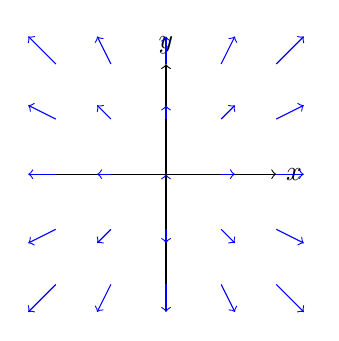
\begin{tikzpicture}[scale=0.7]
\draw[->] (-2,0) -- (2,0) node[right]{$x$};
\draw[->] (0,-2) -- (0,2) node[above]{$y$};
\foreach \x in {-2,...,2} {
    \foreach \y in {-2,...,2} {
        \draw[blue,->] (\x,\y) -- (\x+0.5*\x/2,\y+0.5*\y/2);
    }
}
\end{tikzpicture}
\end{center}

We now compute the flow of $V_1$.

Let $(x_0, y_0)$ be a fixed point in $\mathbb{R}^2$. The flow $\varphi_t$ of $V_1$ satisfies (3) of theorem
\[
\frac{d}{dt} \varphi_t(x_0, y_0) = V_1(\varphi_t(x_0, y_0)).
\]
Here $\varphi_t \colon \mathbb{R}^2 \to \mathbb{R}^2$ is a diffeomorphism for each $t$.

Let $(x(t), y(t))$ be the trajectory followed by $(x_0, y_0)$.
\end{example}

% --- Page 109 ---
In other words, we have the following flow:

\[
(\dot{x}(0), \dot{y}(0)) = (x_0, y_0)
\]
\[
\varphi_t(x_0, y_0) = (x(t), y(t))
\]

Therefore, we have
\[
\frac{d}{dt} \varphi_t(x_0, y_0) = (\dot{x}(t), \dot{y}(t))
\]
where $\dot{}$ represents the derivative with respect to $t$.

By property (3),
\[
(\dot{x}(t), \dot{y}(t)) = V_1(x(t), y(t))
\]
\[
\Rightarrow (\dot{x}(t), \dot{y}(t)) = x(t) \frac{\partial}{\partial x} + y(t) \frac{\partial}{\partial y}
\]

Therefore, we have a system of ordinary differential equations (ODEs) given by
\[
\dot{x}(t) = x(t) \quad \text{and} \quad \dot{y}(t) = y(t)
\]
with the initial condition $x(0) = x_0$ and $y(0) = y_0$.

\begin{proof}
Solving the above system of ODEs, we get
\[
x(t) = x_0 e^{t}, \quad y(t) = y_0 e^{t}
\]
\[
\varphi_t(x_0, y_0) = (x_0 e^{t}, y_0 e^{t}) = e^{t}(x_0, y_0)
\]
\end{proof}

\begin{exercise}
Verify property (2):
\[
\varphi_{t_1 + t_2}(x_0, y_0) = \left(e^{t_1 + t_2} x_0, e^{t_1 + t_2} y_0 \right) = e^{t_1} \left(e^{t_2} x_0, e^{t_2} y_0 \right) = \varphi_{t_1} \circ \varphi_{t_2}(x_0, y_0)
\]
\end{exercise}

% --- Page 110 ---
---

2)

Let \( V_2(x,y) = -y \frac{\partial}{\partial x} + x \frac{\partial}{\partial y} \).

Let \(\varphi_t\) denote the flow of \( V_2 \). Thus,
\[
\varphi_t(x_0, y_0) = (x(t), y(t)) \quad \text{with} \quad x(0) = x_0 \quad \text{and} \quad y(0) = y_0.
\]

Thus,
\[
\frac{d}{dt} \varphi_t(x_0, y_0) = V_2(\varphi_t(x_0, y_0))
\]
implies
\[
(\dot{x}(t), \dot{y}(t)) = (-y(t), x(t)).
\]
Therefore,
\[
\dot{x}(t) = -y(t) \quad \text{and} \quad \dot{y}(t) = x(t).
\]
Differentiating again,
\[
\ddot{x}(t) + x(t) = 0 \quad \text{and} \quad \ddot{y}(t) + y(t) = 0.
\]

Solving the above system, we get
\[
x(t) = x_0 \cos t - y_0 \sin t,
\]
\[
y(t) = x_0 \sin t + y_0 \cos t.
\]

3)

Let \( V_3(x,y) = y \frac{\partial}{\partial x} \).

\[
\frac{d}{dt} \varphi_t(x_0, y_0) = V_3(\varphi_t(x_0, y_0)) = (y(t), 0).
\]
Thus,
\[
\dot{x}(t) = y(t) \implies \ddot{x}(t) = \dot{y}(t) = 0,
\]
and
\[
\dot{y}(t) = 0 \implies y(t) = y_0.
\]
Therefore,
\[
x(t) = y_0 t + x_0,
\]
and
\[
\varphi_t(x_0, y_0) = (y_0 t + x_0, y_0).
\]

% --- Page 111 ---
\begin{theorem}\label{thm:flow_existence_compact}
Let $X$ be a smooth manifold of dimension $n$. Assume that $X$ is a compact manifold (without boundary). Then for every vector field $V$ on $X$, the flow $\varphi_t$ for $V$ exists for all $t \in \mathbb{R}$ with $t \geq 0$.
\end{theorem}

\begin{theorem}\label{thm:flow_existence_uniform}
(This part works for non-compact manifolds.)

If a vector field $V$ on $X$ has the property that the flow of $V$, if it exists, then it exists for $\varepsilon$-time around uniformly each point $x \in X$. Then the flow $\varphi_t$ of $V$ exists for all time $t \in \mathbb{R}$.
\end{theorem}

% --- Page 112 ---
Note that we have an isomorphism
\[ d\varphi_t \colon T_p M \to T_{\varphi_t(p)} M. \]

This motivates the following definition of the rate of change of $\beta$ along the flow of $V$.

Let us denote
\[ \beta_{\varphi_t(p)} \left( d\varphi_t(\cdot), \dots, d\varphi_t(\cdot) \right) \]
by $\varphi_t^* \beta$.

The form $\varphi_t^* \beta$ is called the pullback of $\beta$ via $\varphi_t$.

\begin{definition}\label{def:rate_of_change}
The rate of change of $\beta$ is defined as
\[ \lim_{t \to 0} \frac{\varphi_t^* \beta - \beta}{t}. \]
\end{definition}

% --- Page 113 ---
---

Suppose a $k$-form $\beta$ is given on $X$. We would like to find how $\beta$ changes under the flow of a vector field $V$. (We denote the flow of $V$ by $\varphi_t$.)

Initially, $\beta$ is defined as
\[
\beta_p \colon T_p X \times \cdots \times T_p X \to \mathbb{R}.
\]

After the application of flows, we have
\[
\beta_{\varphi_t(p)} \colon T_{\varphi_t(p)} X \times \cdots \times T_{\varphi_t(p)} X \to \mathbb{R}.
\]

\begin{definition}\label{def:lie_derivative_form}
The rate of change of $\beta$ under the flow of $V$ is given by the Lie derivative of $\beta$ with respect to $V$, defined as
\[
\mathcal{L}_V \beta := \lim_{h \to 0} \frac{\varphi_h^* \beta - \beta}{h},
\]
for the rate of change of $\beta$ at time $t$. This is called the Lie derivative of $\beta$ with respect to the vector field $V$.
\end{definition}

% --- Page 114 ---
\begin{example}\label{ex:lie_derivative_computation}

Let $X = \mathbb{R}^2$ with $(x, y)$ coordinates. Define the vector field
\[
V_1(x, y) = x \frac{\partial}{\partial x} + y \frac{\partial}{\partial y}.
\]
Let $\varphi_t(x_0, y_0) = e^t(x_0, y_0)$. Take the 1-form
\[
\beta_{x,y} = x \, dx + y \, dy.
\]

The differential of $\varphi_t$ is given by
\[
d\varphi_t = \begin{bmatrix}
e^t & 0 \\
0 & e^t
\end{bmatrix}.
\]

Compute the Lie derivative $L_{V_1}\beta$.

First, compute $\varphi_t^*\beta = \beta_{\varphi_t(x_0,y_0)} \circ (d\varphi_t(\cdot))$. Specifically,
\[
\varphi_t^*\beta\left(\frac{\partial}{\partial x}\right) = \beta_{\varphi_t(x_0,y_0)}\left(d\varphi_t\left(\frac{\partial}{\partial x}\right)\right) = e^t \beta_{(x_0,y_0)}\left(\frac{\partial}{\partial x}\right).
\]

Explicitly,
\[
\varphi_t^*\beta\left(\frac{\partial}{\partial x}\right) = e^t \left(e^t x_0 \, dx + e^t y_0 \, dy\right)\left(\frac{\partial}{\partial x}\right) = e^{2t} x_0.
\]

Similarly,
\[
\varphi_t^*\beta\left(\frac{\partial}{\partial y}\right) = e^{2t} y_0.
\]

\end{example}

% --- Page 115 ---
\[
L_{v_1} B \left( \frac{\partial}{\partial x} \right) = \lim_{h \to 0} \frac{\varphi_{t+h}^* B - \varphi_t^* B}{h} \left( \frac{\partial}{\partial x} \right)
\]

\[
= \lim_{h \to 0} \frac{e^{2t+h} x_0 - e^{2t} x_0}{h}
\]

\[
= \lim_{h \to 0} e^{2t} x_0 \left( \frac{e^{2h} - 1}{h} \right)
\]

\[
= e^{2t} x_0 \cdot 2
\]

\[
L_{v_1} B \left( \frac{\partial}{\partial y} \right) = 2 e^{2t} y_0
\]

In particular, Lie derivatives at \( t = 0 \) is given by

\[
L_{v_1} B \left( \frac{\partial}{\partial x} \right) \bigg|_{t=0} = 2 x_0
\]

\[
L_{v_1} B \left( \frac{\partial}{\partial y} \right) \bigg|_{t=0} = 2 y_0
\]

\[
L_{v_1} B = 2 x_0 \, dx + 2 y_0 \, dy.
\]

% --- Page 116 ---
Let $M$ be a smooth manifold of dimension $n$.

\begin{definition}\label{def:contraction}
Let $X$ be a vector field on $M$. The contraction of a $k$-form $\beta$ along $X$ is defined as follows:

The map
\[
i_X: \Omega^k \to \Omega^{k-1}
\]
is given by
\[
i_X \beta \in \Omega^{k-1}.
\]

For $\beta \in \Omega^k(M)$, the contraction $i_X \beta$ is defined on $(v_1, \dots, v_{k-1}) \in T_p M \times \cdots \times T_p M$ by
\[
i_X \beta(v_1, \dots, v_{k-1}) = \beta(X, v_1, \dots, v_{k-1}).
\]
\end{definition}

\begin{remark}\label{rem:linearity}
Check linearity of $i_X$.
\end{remark}

\begin{example}\label{ex:contraction}
Consider $\mathbb{R}^2$ with coordinates $(x, y)$. Let $\omega = dx \wedge dy$. Compute $i_X \omega$ where $X = y \frac{\partial}{\partial x}$.

Let $v \in T_p \mathbb{R}^2$. Then,
\[
i_X \omega(v) = \omega(X, v) = \omega\left(y \frac{\partial}{\partial x}, v\right).
\]
\end{example}

% --- Page 117 ---
\[
= dx \wedge dy \left( y \frac{\partial}{\partial x}, \nu \right) = c_1 dx + c_2 dy
\]

Now, for \(\nu = e_1 = (1, 0)\), \(e_2 = (0, 1)\),

\[
dx \wedge dy \left( y \frac{\partial}{\partial x}, \frac{\partial}{\partial x} \right) dx + dx \wedge dy \left( y \frac{\partial}{\partial x}, \frac{\partial}{\partial y} \right) dy
\]

\[
= \begin{vmatrix} y & 1 \\ 0 & 0 \end{vmatrix} dx + \begin{vmatrix} y & 0 \\ 0 & 1 \end{vmatrix} dy
\]

\[
= y \, dy.
\]

Now take \(X = -y \frac{\partial}{\partial x} + x \frac{\partial}{\partial y}\).

By definition,

\[
i_X (dx \wedge dy) = c_1 dx + c_2 dy
\]

where
\[
c_1 = dx \wedge dy \left( X, \frac{\partial}{\partial x} \right),
\]
\[
c_2 = dx \wedge dy \left( X, \frac{\partial}{\partial y} \right).
\]

\begin{proof}
\[
i_X (dx \wedge dy) = -x \, dx - y \, dy.
\]
\end{proof}

% --- Page 118 ---
Cartan's magic formula states the following:

\[
\mathcal{L}_X \beta = d(i_X \beta) + i_X (d\beta)
\]

for any $k$-form $\beta$ on $M$.

We apply Cartan's Magic Formula to compute $\mathcal{L}_X (d x \wedge d y)$:

\[
\mathcal{L}_y \frac{\partial}{\partial x} = d \left( i_y \frac{\partial}{\partial x} (d x \wedge d y) \right) + i_y d \left( d x \wedge d y \right)
\]

\[
= d(y \, dy) = dy \wedge dy = 0.
\]

---
Exercise: Cartan's Magic Formula on all of the Lie derivatives so far.

Compute $\mathcal{L}_{\partial_x} (d x \wedge d y)$.

Compute $\mathcal{L}_{\partial_x} \left( \sum_{i=1}^n d x_i \wedge d y \right)$ (Use the fact that $i_X$ is a linear operator).

Compute $\mathcal{L}_{\partial x_i} (d x \wedge d y_1 \wedge \cdots \wedge d y_n)$.

\[
d (d x \wedge \cdots \wedge d y_n) = 0
\]

\[
i_{\partial x_i} (d x \wedge d y_1 \wedge \cdots \wedge d y_n) = d x_i \wedge d y_1 \wedge \cdots \wedge \widehat{d y_i} \wedge \cdots \wedge d y_n \quad (\partial x_i, \ldots)
\]

% --- Page 119 ---
The only non-zero $\det(\partial y_1, \ldots, \partial y_n) = 1$

and $d(\overline{I}_{y_1}(d x_1, \ldots, d x_n)) = 0$.

% --- Page 120 ---
\begin{proposition}\label{prop:invariance_of_kform}
Let $M$ be a smooth manifold, for a $k$-form $\beta$ and vector field $X$ on $M$. Then, the flow $\varphi_t$ of $X$ keeps $\beta$ invariant. In other words, $\varphi_t^* \beta = \beta$ $\forall t$.
\end{proposition}

\begin{theorem}[Liouville's Theorem (stronger)]\label{thm:liouville_stronger}
\begin{enumerate}
    \item Let $(M, \omega)$ be a symplectic manifold of dimension $2n$.
    \item Let $H: M \to \mathbb{R}$ be a smooth function.
\end{enumerate}
Then, the flow associated to the Hamiltonian vector field $X_H$ keeps $\omega$ invariant, i.e. if $\varphi_t$ denotes the flow of $X_H$, then
\[
\varphi_t^* \omega = \omega \quad \forall t.
\]
\end{theorem}

% --- Page 121 ---
\begin{proof}
It is sufficient (in light of the proposition) to show
\[
\mathcal{L}_{X_H} \omega = 0.
\]
By Cartan's Magic formula,
\[
\mathcal{L}_{X_H} \omega = d(i_{X_H} \omega) + i_{X_H} d\omega
\]
\[
\implies \mathcal{L}_{X_H} \omega = d(i_{X_H} \omega).
\]
Recall that $i_{X_H} \omega = \omega(X_H, \cdot) = dH(\cdot)$ by the defining property of $X_H$.

\[
\implies \mathcal{L}_{X_H} \omega = d(i_{X_H} \omega) = d(dH) = 0.
\]
\end{proof}

\begin{example}\label{ex:illustration}
Take $M = \mathbb{R}^2$, $\omega = dp \wedge dq$ on
\[
T^* \mathbb{R}^2 = \{(q, p) \mid p, q \in \mathbb{R}\}
\]
and consider
\[
H(p, q) = \frac{1}{2}(p^2 + q^2).
\]
Then,
\[
dH = p \, dp + q \, dq.
\]
\end{example}

% --- Page 122 ---
Therefore, the Hamiltonian vector field is given by
\[ X_H = -p \frac{\partial}{\partial q} + q \frac{\partial}{\partial p}. \]

The flow of the Hamiltonian system is given by
\[ \varphi_t(q, p) = (q \cos t - p \sin t, q \sin t + p \cos t). \]

Let \( M = S^2 = \{(x, y, z) \in \mathbb{R}^3 \mid x^2 + y^2 + z^2 = 1\} \).

Consider the symplectic form given by the area form
\[ \omega \text{ for any } u, v \in T_p S^2 \]
\[ \omega(u, v) = (u \times v) \cdot p. \]

Take \( H: S^2 \to \mathbb{R} \)
\[ H(x, y, z) = z. \]

Compute
\begin{enumerate}
    \item \( dH = dz \in \Omega^1(S^2) \)
    \item \( X_H = \ ? \)
    \item \( \varphi_t = \ ? \)
\end{enumerate}

% --- Page 123 ---
---
By the equality \( w(X_h, \cdot) = dH(\cdot) \),
\[
\omega(X_h|_{c_0, 0, 1}, \cdot) = dz \Big|_{(c_0, 0, 1)} = 0.
\]
By non-degeneracy, \( X_h |_{(c_0, 0, 1)} = 0 \).

\begin{proof}
Suppose \( p = (x_0, y_0, z_0) \). Then
\[
T_p S^2 = \{(u, v, w) \mid (u, v, w) \cdot (x_0, y_0, z_0) = 0\}.
\]
Now, \( dz \colon T_p S^2 \to \mathbb{R} \) is defined by
\[
(u, v, w) \mapsto w.
\]

We have
\[
dz(u \, d x + v \, d y + w \, d z) = w.
\]
Therefore,
\[
\omega(X_h, u \, d x + v \, d y + w \, d z) = dz(u \, d x + v \, d y + w \, d z) = w.
\]
This implies
\[
(X_h \times (u \, d x + v \, d y + w \, d z)) \cdot (x_0 \, d x + y_0 \, d y + z_0 \, d z) = w.
\]

Let \( X_h = c_1 \, d x + c_2 \, d y + c_3 \, d z \). Then
\[
X_h \times (u \, d x + v \, d y + w \, d z) = (c_2 w - c_3 v) \, d x - (c_1 w - c_3 u) \, d y + (c_1 v - c_2 u) \, d z.
\]
\end{proof}
---

% --- Page 124 ---
The handwritten content does not explicitly contain labeled definitions, theorems, lemmas, or proofs, but it does contain a sequence of mathematical derivations and statements. 
---

We have the following equation:
\[
\left( X_n \times (u\,dx + v\,dy + w\,dz) \right) \cdot \left( x_0\,dx + y_0\,dy + z_0\,dz \right) = w.
\]

This simplifies to:
\[
x_0 (c_2 w - c_3 v) - y_0 (c_1 w - c_3 u) + z_0 (c_1 v - c_2 u) = w.
\]

The equation is satisfied by all $(u, v, w) \in T_p S^2$.

\begin{definition}\label{def:choice}
Take $(u, v, w) = (-y_0, x_0, 0)$ as it satisfies (*).
\end{definition}

Substituting the above choice, we get:
\[
x_0 \left( -c_3 x_0 \right) - y_0 \left( -c_3 (-y_0) \right) + z_0 \left( c_1 x_0 + c_2 y_0 \right) = 0.
\]

Simplifying, we obtain:
\[
-c_3 x_0^2 - c_3 y_0^2 + z_0 (c_1 x_0 + c_2 y_0) = 0.
\]

Change point to get 3 equations and find $c_1, c_2, c_3$.

---

% --- Page 125 ---
Given a symplectic form $(M, \omega)$, we have a natural choice of volume form, i.e. $2n$-form, given by

\[
\omega^n = \underbrace{\omega \wedge \omega \cdots \wedge \omega}_{n \text{ form wedge product}}.
\]

\begin{exercise}
On $\mathbb{R}^4$ consider $\omega = dq_1 \wedge dp_1 + dq_2 \wedge dp_2$ with coordinate system $(q_1, q_2, p_1, p_2)$.

Here $\omega^2 = (dq_1 \wedge dp_1 + dq_2 \wedge dp_2)^2$

\[
= dq_1 \wedge dp_1 \wedge dq_1 \wedge dp_1 + dq_2 \wedge dp_2 \wedge dq_2 \wedge dp_2
\]

\[
+ dq_1 \wedge dp_1 \wedge dq_2 \wedge dp_2 + dq_2 \wedge dp_2 \wedge dq_1 \wedge dp_1.
\]

Now $dq_2 \wedge dp_2 \wedge dq_1 \wedge dp_1 = dq_1 \wedge dp_1 \wedge dq_2 \wedge dp_2$.

Hence

\[
\omega^2 = 2 \cdot dq_1 \wedge dp_1 \wedge dq_2 \wedge dp_2.
\]
\end{exercise}

% --- Page 126 ---
In general on $\mathbb{R}^{2n}$ with coordinates
$(q_1, \dots, q_n, p_1, \dots, p_n)$
and $\omega = \sum_{i=1}^n dq_i \wedge dp_i$.

Compute:
\[
\omega^n = \left(\sum_{i=1}^n dq_i \wedge dp_i\right)^n = n! \, (dq_1 \wedge dp_1) \wedge \cdots \wedge (dq_n \wedge dp_n)
\]

In general, the $2n$-form $\omega^k$ does not vanish at any point of $M$.

\[
\omega^k : T_p M \times \cdots \times T_p M \to \mathbb{R}.
\]

Suppose at $p$, $\omega^n = 0$.

\[
\omega^n(v_1, \dots, v_{2n}) = 0 \quad \forall v_i \in T_p M.
\]

Take a symplectic basis of a symplectic vector space.
$(T_p M, \omega_p)$ denote it by $(e_1, \dots, e_n, f_1, \dots, f_n)$,
\[
\omega_p(e_i, e_j) = \omega(f_i, f_j) = 0,
\]
\[
\omega(e_i, f_j) = \delta_{ij}.
\]

\[
(\omega \wedge \cdots \wedge \omega)(e_1, \dots, e_n, f_1, \dots, f_n) \neq 0.
\]

(Verify the computation.)

% --- Page 127 ---
Therefore, $w^n$ at any point $p$ is a non-zero $2n$-form.

On symplectic manifold $(M, \omega)$, the $2n$-form $w^n$ gives us a volume.

\begin{theorem}[Liouville's Theorem (Weak form)]
The setup is the same as strong form. Then the flow $\varphi_{X_H}$ associated to $H$ preserves the volume form $w^n$. In other words,
\[
\mathcal{L}_{X_H} w^n = 0.
\]
\end{theorem}

\begin{proof}
Strong form $\implies$ Weak form
\[
\varphi_t^* w = w \quad \text{for all } t
\]
Observe
\[
\varphi^* (w \wedge \cdots \wedge w) = (\varphi^* w)^n
\]
where the left-hand side is an $n$-form.

Prove it yourself.
\end{proof}

% --- Page 128 ---
Consider $\mathbb{R}^2$ with $q, p_1$ coordinates.

Let $H: \mathbb{R}^2 \to \mathbb{R}$ be a smooth function

\[
\begin{proof}
\text{If } A \text{ is a region in } \mathbb{R}^2, \text{ then the area of } A \text{ is preserved under the flow of Hamiltonian vector field } X_H.
\end{proof}
\]

% --- Page 129 ---
% blank page

% --- Page 130 ---
% blank page

% --- Page 131 ---
% blank page

% --- Page 132 ---
% blank page

\end{document}